\documentclass{article}\usepackage[]{graphicx}\usepackage[]{color}
%% maxwidth is the original width if it is less than linewidth
%% otherwise use linewidth (to make sure the graphics do not exceed the margin)
\makeatletter
\def\maxwidth{ %
  \ifdim\Gin@nat@width>\linewidth
    \linewidth
  \else
    \Gin@nat@width
  \fi
}
\makeatother

\definecolor{fgcolor}{rgb}{0.345, 0.345, 0.345}
\newcommand{\hlnum}[1]{\textcolor[rgb]{0.686,0.059,0.569}{#1}}%
\newcommand{\hlstr}[1]{\textcolor[rgb]{0.192,0.494,0.8}{#1}}%
\newcommand{\hlcom}[1]{\textcolor[rgb]{0.678,0.584,0.686}{\textit{#1}}}%
\newcommand{\hlopt}[1]{\textcolor[rgb]{0,0,0}{#1}}%
\newcommand{\hlstd}[1]{\textcolor[rgb]{0.345,0.345,0.345}{#1}}%
\newcommand{\hlkwa}[1]{\textcolor[rgb]{0.161,0.373,0.58}{\textbf{#1}}}%
\newcommand{\hlkwb}[1]{\textcolor[rgb]{0.69,0.353,0.396}{#1}}%
\newcommand{\hlkwc}[1]{\textcolor[rgb]{0.333,0.667,0.333}{#1}}%
\newcommand{\hlkwd}[1]{\textcolor[rgb]{0.737,0.353,0.396}{\textbf{#1}}}%

\usepackage{framed}
\makeatletter
\newenvironment{kframe}{%
 \def\at@end@of@kframe{}%
 \ifinner\ifhmode%
  \def\at@end@of@kframe{\end{minipage}}%
  \begin{minipage}{\columnwidth}%
 \fi\fi%
 \def\FrameCommand##1{\hskip\@totalleftmargin \hskip-\fboxsep
 \colorbox{shadecolor}{##1}\hskip-\fboxsep
     % There is no \\@totalrightmargin, so:
     \hskip-\linewidth \hskip-\@totalleftmargin \hskip\columnwidth}%
 \MakeFramed {\advance\hsize-\width
   \@totalleftmargin\z@ \linewidth\hsize
   \@setminipage}}%
 {\par\unskip\endMakeFramed%
 \at@end@of@kframe}
\makeatother

\definecolor{shadecolor}{rgb}{.97, .97, .97}
\definecolor{messagecolor}{rgb}{0, 0, 0}
\definecolor{warningcolor}{rgb}{1, 0, 1}
\definecolor{errorcolor}{rgb}{1, 0, 0}
\newenvironment{knitrout}{}{} % an empty environment to be redefined in TeX

\usepackage{alltt}
\usepackage{geometry}
\usepackage{amsmath}
\usepackage{lscape}
\geometry{verbose,tmargin=2.5cm,bmargin=2.5cm,lmargin=2.5cm,rmargin=2.5cm}
\IfFileExists{upquote.sty}{\usepackage{upquote}}{}
\begin{document}




\begin{knitrout}
\definecolor{shadecolor}{rgb}{0.969, 0.969, 0.969}\color{fgcolor}\begin{kframe}
\begin{alltt}
\hlkwd{library}\hlstd{(flexsurv)}
\end{alltt}


{\ttfamily\noindent\itshape\color{messagecolor}{\#\# Loading required package: survival\\\#\# Loading required package: splines}}\begin{alltt}
\hlkwd{library}\hlstd{(boot)}
\end{alltt}


{\ttfamily\noindent\itshape\color{messagecolor}{\#\# \\\#\# Attaching package: 'boot'\\\#\# \\\#\# The following object is masked from 'package:survival':\\\#\# \\\#\#\ \ \ \  aml}}\begin{alltt}
\hlkwd{library}\hlstd{(randomForestSRC)}
\end{alltt}


{\ttfamily\noindent\itshape\color{messagecolor}{\#\# Loading required package: parallel\\\#\# \\\#\#\ \ randomForestSRC 1.5.5 \\\#\#\ \ \\\#\#\ \ Type rfsrc.news() to see new features, changes, and bug fixes. \\\#\# }}\begin{alltt}
\hlkwd{library}\hlstd{(timeROC)}
\end{alltt}


{\ttfamily\noindent\itshape\color{messagecolor}{\#\# Loading required package: pec\\\#\# Loading required package: mvtnorm\\\#\# Loading required package: timereg}}\begin{alltt}
\hlkwd{library}\hlstd{(risksetROC)}
\end{alltt}


{\ttfamily\noindent\itshape\color{messagecolor}{\#\# Loading required package: MASS}}\begin{alltt}
\hlkwd{library}\hlstd{(RColorBrewer)}
\hlstd{pal} \hlkwb{=} \hlkwd{brewer.pal}\hlstd{(}\hlnum{6}\hlstd{,} \hlstr{"Dark2"}\hlstd{)}
\hlkwd{names}\hlstd{(pal)} \hlkwb{=} \hlkwd{c}\hlstd{(}\hlstr{"gg"}\hlstd{,} \hlstr{"cph"}\hlstd{,} \hlstr{"rsf"}\hlstd{,} \hlstr{"km0"}\hlstd{,} \hlstr{"mskcc.pre"}\hlstd{,} \hlstr{"mskcc.post"}\hlstd{)}
\end{alltt}
\end{kframe}
\end{knitrout}


\section{Preparation}
Construct a *preoperative* function based on the Brennan nomogram.  The preoperative nature will mean that most prognostic components will need to be marginalized out.

\begin{table}[h]
\begin{tabular}{llll}
Variable            & Preoperative? & Available? & Marginals                                                                                     \\
Age                 & Yes           & Yes        & Linear.  90 =\textgreater 0, 30 =\textgreater 8.  Therefore $f(x) = -2/15(x-90) = -2/15x + 12$ \\
Sex                 & Yes           & Yes        & Male risk delta 3                                                                             \\
Portal Vein         & NO            &            & 14.4\% YES, risk delta 10, marginal 1.4                                                       \\
Splenectomy         & NO            &            & 9.9\% YES, risk delta 62, marginal 6.1                                                        \\
Margin of resection & NO            &            & 20.7\% POS, risk delta 4, marginal 0.8                                                        \\
Head.vs.Other       & Yes           & Yes        & Head risk delta 51                                                                            \\
Differentiation     & NO            &            & 14.2\% Well, risk delta 0, marginal 0                                                         \\
                    &               &            & 56.4\% Mod, risk delta 14, marginal 7.9                                                       \\
                    &               &            & 29.5\% Poor, risk delta 35, marginal 10.3.  Overall marginal 18.2                             \\
Posterior.margin    & NO            &            & 86.0\% POS, risk delta 22, marginal 18.9                                                      \\
Numb.pos.nodes      & NO            &            & Mean 2.1, approx marginal 15                                                                  \\
Numb.neg.nodes      & NO            &            & Mean 16.9, approx marginal 9                                                                  \\
Back.pain           & Yes           & NO         & 13.7\% YES, risk delta 15, marginal 2.0                                                       \\
T.stage             & Yes           & Yes        &                                                                                               \\
Weight Loss         & Yes           & NO         & 53.7\% YES, risk delta 3,  marginal 1.6                                                       \\
Max.path.axis       & Yes           & Yes        &                                                                                              
\end{tabular}
\end{table}

So the preoperative MSKCC score would be:
\begin{align}
S &= 1.4 + 6.1 + 0.8 + 18.2 + 18.9 + 15 + 9 + 15*Back.pain + 3*Weight.Loss + -2/15*Age + 12 + 3\left[Sex = M\right] + 51\left[Head.vs.Other = Head\right] + T.stage + Max.path.axis
  &= 81.4 + 15*Back.pain + 3*Weight.Loss + -2/15*Age + 3*\left[Sex = M\right] + 51\left[Head.vs.Other = Head\right] + fT(T.stage) + fS(Max.path.axis)
fT(T.stage) = 36\left[T.stage = T1\right] + 10\left[T.stage = T3\right] + 63\left[T.stage = T4\right]
\end{align}


\begin{knitrout}
\definecolor{shadecolor}{rgb}{0.969, 0.969, 0.969}\color{fgcolor}\begin{kframe}
\begin{alltt}
\hlstd{fit.mskcc} \hlkwb{=} \hlkwd{list}\hlstd{(}
        \hlkwc{inputs} \hlstd{=} \hlkwd{list}\hlstd{(}
        \hlkwc{History.Diagnosis.AgeAt} \hlstd{=} \hlkwd{list}\hlstd{(}
                \hlkwc{margins} \hlstd{=} \hlkwd{data.frame}\hlstd{(}\hlkwc{value} \hlstd{=} \hlnum{65}\hlstd{,} \hlkwc{fraction} \hlstd{=} \hlnum{1}\hlstd{),}
                \hlkwc{scorefunc} \hlstd{=} \hlkwa{function}\hlstd{(}\hlkwc{x}\hlstd{) \{ x} \hlkwb{=} \hlstd{x;} \hlopt{-}\hlnum{2}\hlopt{/}\hlnum{15}\hlopt{*}\hlkwd{pmin}\hlstd{(}\hlkwd{pmax}\hlstd{(x,} \hlnum{0}\hlstd{),} \hlnum{90}\hlstd{)} \hlopt{+} \hlnum{12} \hlstd{\}),}
        \hlkwc{Patient.Sex} \hlstd{=} \hlkwd{list}\hlstd{(}
                \hlkwc{margins} \hlstd{=} \hlkwd{data.frame}\hlstd{(}\hlkwc{value} \hlstd{=} \hlkwd{c}\hlstd{(}\hlstr{"M"}\hlstd{,} \hlstr{"F"}\hlstd{),} \hlkwc{fraction} \hlstd{=} \hlkwd{c}\hlstd{(}\hlnum{0.501}\hlstd{,} \hlnum{1}\hlopt{-}\hlnum{0.501}\hlstd{)),}
                \hlkwc{scorefunc} \hlstd{=} \hlkwa{function}\hlstd{(}\hlkwc{x}\hlstd{) \{} \hlnum{3}\hlopt{*}\hlkwd{I}\hlstd{(x} \hlopt{==} \hlstr{"M"}\hlstd{) \}),}
        \hlkwc{Portal.Vein} \hlstd{=} \hlkwd{list}\hlstd{(}
                \hlkwc{margins} \hlstd{=} \hlkwd{data.frame}\hlstd{(}\hlkwc{value} \hlstd{=} \hlkwd{c}\hlstd{(}\hlnum{TRUE}\hlstd{,} \hlnum{FALSE}\hlstd{),} \hlkwc{fraction} \hlstd{=} \hlkwd{c}\hlstd{(}\hlnum{0.144}\hlstd{,} \hlnum{1}\hlopt{-}\hlnum{0.144}\hlstd{)),}
                \hlkwc{scorefunc} \hlstd{=} \hlkwa{function}\hlstd{(}\hlkwc{x}\hlstd{) \{} \hlnum{10}\hlopt{*}\hlkwd{I}\hlstd{(x} \hlopt{==} \hlnum{TRUE}\hlstd{) \}),}
        \hlkwc{Splenectomy} \hlstd{=} \hlkwd{list}\hlstd{(}
                \hlkwc{margins} \hlstd{=} \hlkwd{data.frame}\hlstd{(}\hlkwc{value} \hlstd{=} \hlkwd{c}\hlstd{(}\hlnum{TRUE}\hlstd{,} \hlnum{FALSE}\hlstd{),} \hlkwc{fraction} \hlstd{=} \hlkwd{c}\hlstd{(}\hlnum{0.099}\hlstd{,} \hlnum{1}\hlopt{-}\hlnum{0.099}\hlstd{)),}
                \hlkwc{scorefunc} \hlstd{=} \hlkwa{function}\hlstd{(}\hlkwc{x}\hlstd{) \{} \hlnum{62}\hlopt{*}\hlkwd{I}\hlstd{(x} \hlopt{==} \hlnum{TRUE}\hlstd{) \}),}
        \hlkwc{Treat.MarginPositive} \hlstd{=} \hlkwd{list}\hlstd{(}
                \hlkwc{margins} \hlstd{=} \hlkwd{data.frame}\hlstd{(}\hlkwc{value} \hlstd{=} \hlkwd{c}\hlstd{(}\hlnum{TRUE}\hlstd{,} \hlnum{FALSE}\hlstd{),} \hlkwc{fraction} \hlstd{=} \hlkwd{c}\hlstd{(}\hlnum{0.207}\hlstd{,} \hlnum{1}\hlopt{-}\hlnum{0.207}\hlstd{)),}
                \hlkwc{scorefunc} \hlstd{=} \hlkwa{function}\hlstd{(}\hlkwc{x}\hlstd{) \{} \hlnum{4}\hlopt{*}\hlkwd{I}\hlstd{(x} \hlopt{==} \hlnum{TRUE}\hlstd{) \}),}
        \hlkwc{Path.LocationBody} \hlstd{=} \hlkwd{list}\hlstd{(}
                \hlkwc{margins} \hlstd{=} \hlkwd{data.frame}\hlstd{(}\hlkwc{value} \hlstd{=} \hlkwd{c}\hlstd{(}\hlnum{FALSE}\hlstd{,} \hlnum{TRUE}\hlstd{),} \hlkwc{fraction} \hlstd{=} \hlkwd{c}\hlstd{(}\hlnum{0.894}\hlstd{,} \hlnum{1}\hlopt{-}\hlnum{0.894}\hlstd{)),}
                \hlkwc{scorefunc} \hlstd{=} \hlkwa{function}\hlstd{(}\hlkwc{x}\hlstd{) \{} \hlnum{51}\hlopt{*}\hlkwd{I}\hlstd{(x} \hlopt{==} \hlnum{TRUE}\hlstd{) \}),}
        \hlkwc{Path.Differentiation} \hlstd{=} \hlkwd{list}\hlstd{(}
                \hlkwc{margins} \hlstd{=} \hlkwd{data.frame}\hlstd{(}\hlkwc{value} \hlstd{=} \hlkwd{c}\hlstd{(}\hlstr{"1"}\hlstd{,} \hlstr{"2"}\hlstd{,} \hlstr{"3"}\hlstd{,} \hlstr{"4"}\hlstd{),} \hlkwc{fraction} \hlstd{=} \hlkwd{c}\hlstd{(}\hlnum{0.142}\hlstd{,} \hlnum{0.564}\hlstd{,} \hlnum{1}\hlopt{-}\hlnum{0.142}\hlopt{-}\hlnum{0.564}\hlstd{,} \hlnum{0}\hlstd{)),}
                \hlkwc{scorefunc} \hlstd{=} \hlkwa{function}\hlstd{(}\hlkwc{x}\hlstd{) \{} \hlnum{14}\hlopt{*}\hlkwd{I}\hlstd{(x} \hlopt{==} \hlstr{"2"}\hlstd{)} \hlopt{+} \hlnum{35}\hlopt{*}\hlkwd{I}\hlstd{(x} \hlopt{==} \hlstr{"3"}\hlstd{)} \hlopt{+} \hlnum{35}\hlopt{*}\hlkwd{I}\hlstd{(x} \hlopt{==} \hlstr{"4"}\hlstd{) \}),}          \hlcom{# Undifferentiated (4) not covered by the MSKCC nomogram; here assign the same score as poorly differentiated (3)}
        \hlkwc{Posterior.Margin} \hlstd{=} \hlkwd{list}\hlstd{(}
                \hlkwc{margins} \hlstd{=} \hlkwd{data.frame}\hlstd{(}\hlkwc{value} \hlstd{=} \hlkwd{c}\hlstd{(}\hlnum{TRUE}\hlstd{,} \hlnum{FALSE}\hlstd{),} \hlkwc{fraction} \hlstd{=} \hlkwd{c}\hlstd{(}\hlnum{0.86}\hlstd{,} \hlnum{1}\hlopt{-}\hlnum{0.86}\hlstd{)),}
                \hlkwc{scorefunc} \hlstd{=} \hlkwa{function}\hlstd{(}\hlkwc{x}\hlstd{) \{} \hlnum{22}\hlopt{*}\hlkwd{I}\hlstd{(x} \hlopt{==} \hlnum{TRUE}\hlstd{) \}),}
        \hlkwc{Path.LN.Involved} \hlstd{=} \hlkwd{list}\hlstd{(}
                \hlkwc{margins} \hlstd{=} \hlkwd{data.frame}\hlstd{(}\hlkwc{value} \hlstd{=} \hlnum{2.1}\hlstd{,} \hlkwc{fraction} \hlstd{=} \hlnum{1}\hlstd{),}
                \hlkwc{scorefunc} \hlstd{=} \hlkwa{function}\hlstd{(}\hlkwc{x}\hlstd{) \{}
                        \hlstd{x} \hlkwb{=} \hlkwd{pmin}\hlstd{(}\hlnum{40}\hlstd{,} \hlkwd{pmax}\hlstd{(x,} \hlnum{0}\hlstd{))}
                        \hlstd{fitfun} \hlkwb{=} \hlkwd{splinefun}\hlstd{(}\hlkwd{c}\hlstd{(}\hlnum{0}\hlstd{,} \hlnum{1}\hlstd{,} \hlnum{2}\hlstd{,} \hlnum{3}\hlstd{,} \hlnum{4}\hlstd{,} \hlnum{10}\hlstd{,} \hlnum{15}\hlstd{,} \hlnum{20}\hlstd{,} \hlnum{25}\hlstd{,} \hlnum{30}\hlstd{,} \hlnum{35}\hlstd{,} \hlnum{40}\hlstd{),} \hlkwd{c}\hlstd{(}\hlnum{0}\hlstd{,} \hlnum{14.56}\hlstd{,} \hlnum{24.64}\hlstd{,} \hlnum{30.28}\hlstd{,} \hlnum{33.00}\hlstd{,} \hlnum{39.05}\hlstd{,} \hlnum{43.89}\hlstd{,} \hlnum{48.83}\hlstd{,} \hlnum{53.77}\hlstd{,} \hlnum{58.61}\hlstd{,} \hlnum{63.55}\hlstd{,} \hlnum{68.49}\hlstd{),} \hlkwc{method} \hlstd{=} \hlstr{"natural"}\hlstd{)}
                        \hlkwd{fitfun}\hlstd{(x)}
                \hlstd{\}),}
        \hlkwc{Path.LN.Negative} \hlstd{=} \hlkwd{list}\hlstd{(}
                \hlkwc{margins} \hlstd{=} \hlkwd{data.frame}\hlstd{(}\hlkwc{value} \hlstd{=} \hlnum{16.9}\hlstd{,} \hlkwc{fraction} \hlstd{=} \hlnum{1}\hlstd{),}
                \hlkwc{scorefunc} \hlstd{=} \hlkwa{function}\hlstd{(}\hlkwc{x}\hlstd{) \{ (}\hlkwd{pmin}\hlstd{(}\hlkwd{pmax}\hlstd{(x,} \hlnum{0}\hlstd{),} \hlnum{90}\hlstd{)}\hlopt{-}\hlnum{90}\hlstd{)}\hlopt{*-}\hlnum{11}\hlopt{/}\hlnum{90} \hlstd{\}),}
        \hlkwc{Back.pain} \hlstd{=} \hlkwd{list}\hlstd{(}
                \hlkwc{margins} \hlstd{=} \hlkwd{data.frame}\hlstd{(}\hlkwc{value} \hlstd{=} \hlkwd{c}\hlstd{(}\hlnum{TRUE}\hlstd{,} \hlnum{FALSE}\hlstd{),} \hlkwc{fraction} \hlstd{=} \hlkwd{c}\hlstd{(}\hlnum{0.137}\hlstd{,} \hlnum{1}\hlopt{-}\hlnum{0.137}\hlstd{)),}
                \hlkwc{scorefunc} \hlstd{=} \hlkwa{function}\hlstd{(}\hlkwc{x}\hlstd{) \{} \hlnum{15}\hlopt{*}\hlkwd{I}\hlstd{(x} \hlopt{==} \hlnum{TRUE}\hlstd{) \}),}
        \hlkwc{Stage.pT.Simplified} \hlstd{=} \hlkwd{list}\hlstd{(}
                \hlkwc{margins} \hlstd{=} \hlkwd{data.frame}\hlstd{(}\hlkwc{value} \hlstd{=} \hlkwd{c}\hlstd{(}\hlstr{"T1"}\hlstd{,} \hlstr{"T2"}\hlstd{,} \hlstr{"T34"}\hlstd{),} \hlkwc{fraction} \hlstd{=} \hlkwd{c}\hlstd{(}\hlnum{0.037}\hlstd{,} \hlnum{0.119}\hlstd{,} \hlnum{1}\hlopt{-}\hlnum{0.037}\hlopt{-}\hlnum{0.119}\hlstd{)),}
                \hlkwc{scorefunc} \hlstd{=} \hlkwa{function}\hlstd{(}\hlkwc{x}\hlstd{) \{} \hlnum{36}\hlopt{*}\hlkwd{I}\hlstd{(x} \hlopt{==} \hlstr{"T1"}\hlstd{)} \hlopt{+} \hlnum{11}\hlopt{*}\hlkwd{I}\hlstd{(x} \hlopt{==} \hlstr{"T34"}\hlstd{) \}),}
                \hlcom{# The following matches the original Brennan nomogram, but was not used as there are too few T4}
                \hlcom{# tumours in either the NSWPCN *or* the MSKCC cohorts -- how the T4 coefficient was ever estimated,}
                \hlcom{# I'll never know.  The T34 coefficient of 11 was arrived at as (0.828*10+(1-0.037-0.119-0.828)*63)/(1-0.037-0.119),}
                \hlcom{# being a frequency-weighted average of the T3 and T4 coefficients.}
                \hlcom{# margins = data.frame(value = c("T1", "T2", "T3", "T4"), fraction = c(0.037, 0.119, 0.828, 1-0.037-0.119-0.828)),}
                \hlcom{# scorefunc = function(x) \{ 36*I(x == "T1") + 10*I(x == "T3") + 63*I(x == "T4") \}),}
        \hlkwc{Weight.loss} \hlstd{=} \hlkwd{list}\hlstd{(}
                \hlkwc{margins} \hlstd{=} \hlkwd{data.frame}\hlstd{(}\hlkwc{value} \hlstd{=} \hlkwd{c}\hlstd{(}\hlnum{TRUE}\hlstd{,} \hlnum{FALSE}\hlstd{),} \hlkwc{fraction} \hlstd{=} \hlkwd{c}\hlstd{(}\hlnum{0.537}\hlstd{,} \hlnum{1}\hlopt{-}\hlnum{0.537}\hlstd{)),}
                \hlkwc{scorefunc} \hlstd{=} \hlkwa{function}\hlstd{(}\hlkwc{x}\hlstd{) \{} \hlnum{3}\hlopt{*}\hlkwd{I}\hlstd{(x} \hlopt{==} \hlnum{TRUE}\hlstd{) \}),}
        \hlkwc{Path.Size} \hlstd{=} \hlkwd{list}\hlstd{(}
                \hlkwc{margins} \hlstd{=} \hlkwd{data.frame}\hlstd{(),}
                \hlkwc{scorefunc} \hlstd{=} \hlkwa{function}\hlstd{(}\hlkwc{x}\hlstd{) \{}
                        \hlstd{x} \hlkwb{=} \hlkwd{pmin}\hlstd{(}\hlnum{16}\hlstd{,} \hlkwd{pmax}\hlstd{(x,} \hlnum{0}\hlstd{))}
                        \hlstd{fitfun} \hlkwb{=} \hlkwd{splinefun}\hlstd{(}\hlkwd{c}\hlstd{(}\hlnum{0}\hlstd{,} \hlnum{1}\hlstd{,} \hlnum{2}\hlstd{,} \hlnum{3}\hlstd{,} \hlnum{4}\hlstd{,} \hlnum{6}\hlstd{,} \hlnum{8}\hlstd{,} \hlnum{10}\hlstd{,} \hlnum{12}\hlstd{,} \hlnum{14}\hlstd{,} \hlnum{16}\hlstd{),} \hlkwd{c}\hlstd{(}\hlnum{0}\hlstd{,} \hlnum{29.74}\hlstd{,} \hlnum{59.48}\hlstd{,} \hlnum{86.70}\hlstd{,} \hlnum{100}\hlstd{,} \hlnum{97.29}\hlstd{,} \hlnum{90.03}\hlstd{,} \hlnum{82.77}\hlstd{,} \hlnum{75.51}\hlstd{,} \hlnum{68.25}\hlstd{,} \hlnum{61.10}\hlstd{),} \hlkwc{method} \hlstd{=} \hlstr{"natural"}\hlstd{)}
                        \hlkwd{fitfun}\hlstd{(x)}
                \hlstd{\}) ),}
        \hlkwc{outputs} \hlstd{=} \hlkwd{list}\hlstd{(}
                \hlkwc{DSS12mo} \hlstd{=} \hlkwa{function}\hlstd{(}\hlkwc{s}\hlstd{) \{}
                        \hlstd{x} \hlkwb{=} \hlkwd{pmax}\hlstd{(}\hlnum{50}\hlstd{,} \hlkwd{pmin}\hlstd{(}\hlnum{350}\hlstd{, s))}
                        \hlstd{fitfun} \hlkwb{=} \hlkwd{splinefun}\hlstd{(}\hlkwd{c}\hlstd{(}\hlnum{79.0323}\hlstd{,} \hlnum{115.02}\hlstd{,} \hlnum{165.524}\hlstd{,} \hlnum{197.278}\hlstd{,} \hlnum{221.774}\hlstd{,} \hlnum{242.339}\hlstd{,} \hlnum{261.089}\hlstd{,} \hlnum{279.839}\hlstd{,} \hlnum{299.194}\hlstd{,} \hlnum{323.992}\hlstd{,} \hlnum{337.298}\hlstd{),} \hlkwd{c}\hlstd{(}\hlnum{0.94}\hlstd{,} \hlnum{0.9}\hlstd{,} \hlnum{0.8}\hlstd{,} \hlnum{0.7}\hlstd{,} \hlnum{0.6}\hlstd{,} \hlnum{0.5}\hlstd{,} \hlnum{0.4}\hlstd{,} \hlnum{0.3}\hlstd{,} \hlnum{0.2}\hlstd{,} \hlnum{0.1}\hlstd{,} \hlnum{0.06}\hlstd{))}
                        \hlstd{y} \hlkwb{=} \hlkwd{fitfun}\hlstd{(x)}
                        \hlkwd{pmax}\hlstd{(}\hlnum{0}\hlstd{,} \hlkwd{pmin}\hlstd{(}\hlnum{1}\hlstd{, y))}
                \hlstd{\},}
                \hlkwc{DSS24mo} \hlstd{=} \hlkwa{function}\hlstd{(}\hlkwc{s}\hlstd{) \{}
                        \hlstd{x} \hlkwb{=} \hlkwd{pmax}\hlstd{(}\hlnum{50}\hlstd{,} \hlkwd{pmin}\hlstd{(}\hlnum{350}\hlstd{, s))}
                        \hlstd{fitfun} \hlkwb{=} \hlkwd{splinefun}\hlstd{(}\hlkwd{c}\hlstd{(}\hlnum{71.1694}\hlstd{,} \hlnum{97.7823}\hlstd{,} \hlnum{129.536}\hlstd{,} \hlnum{153.73}\hlstd{,} \hlnum{174.294}\hlstd{,} \hlnum{193.347}\hlstd{,} \hlnum{211.794}\hlstd{,} \hlnum{231.452}\hlstd{,} \hlnum{255.645}\hlstd{,} \hlnum{303.125}\hlstd{),} \hlkwd{c}\hlstd{(}\hlnum{0.86}\hlstd{,} \hlnum{0.8}\hlstd{,} \hlnum{0.7}\hlstd{,} \hlnum{0.6}\hlstd{,} \hlnum{0.5}\hlstd{,} \hlnum{0.4}\hlstd{,} \hlnum{0.3}\hlstd{,} \hlnum{0.2}\hlstd{,} \hlnum{0.1}\hlstd{,} \hlnum{0.01}\hlstd{))}
                        \hlstd{y} \hlkwb{=} \hlkwd{fitfun}\hlstd{(x)}
                        \hlkwd{pmax}\hlstd{(}\hlnum{0}\hlstd{,} \hlkwd{pmin}\hlstd{(}\hlnum{1}\hlstd{, y))}
                \hlstd{\},}
                \hlkwc{DSS36mo} \hlstd{=} \hlkwa{function}\hlstd{(}\hlkwc{s}\hlstd{) \{}
                        \hlstd{x} \hlkwb{=} \hlkwd{pmax}\hlstd{(}\hlnum{50}\hlstd{,} \hlkwd{pmin}\hlstd{(}\hlnum{350}\hlstd{, s))}
                        \hlstd{fitfun} \hlkwb{=} \hlkwd{splinefun}\hlstd{(}\hlkwd{c}\hlstd{(}\hlnum{69.3548}\hlstd{,} \hlnum{101.109}\hlstd{,} \hlnum{125.302}\hlstd{,} \hlnum{145.867}\hlstd{,} \hlnum{164.919}\hlstd{,} \hlnum{183.367}\hlstd{,} \hlnum{202.722}\hlstd{,} \hlnum{226.915}\hlstd{,} \hlnum{274.093}\hlstd{),} \hlkwd{c}\hlstd{(}\hlnum{0.8}\hlstd{,} \hlnum{0.7}\hlstd{,} \hlnum{0.6}\hlstd{,} \hlnum{0.5}\hlstd{,} \hlnum{0.4}\hlstd{,} \hlnum{0.3}\hlstd{,} \hlnum{0.2}\hlstd{,} \hlnum{0.1}\hlstd{,} \hlnum{0.01}\hlstd{))}
                        \hlstd{y} \hlkwb{=} \hlkwd{fitfun}\hlstd{(x)}
                        \hlkwd{pmax}\hlstd{(}\hlnum{0}\hlstd{,} \hlkwd{pmin}\hlstd{(}\hlnum{1}\hlstd{, y))}
                \hlstd{\})}
        \hlstd{)}

\hlstd{applyNomogram} \hlkwb{=} \hlkwa{function}\hlstd{(}\hlkwc{nomogram}\hlstd{,} \hlkwc{data}\hlstd{)}
\hlstd{\{}
        \hlstd{scores} \hlkwb{=} \hlkwd{rowSums}\hlstd{(}\hlkwd{sapply}\hlstd{(}\hlkwd{names}\hlstd{(nomogram}\hlopt{$}\hlstd{inputs),} \hlkwa{function}\hlstd{(}\hlkwc{input}\hlstd{) \{}
                \hlkwa{if} \hlstd{(input} \hlopt \hlkwd{colnames}\hlstd{(data)) \{}
                        \hlkwd{return}\hlstd{(nomogram}\hlopt{$}\hlstd{inputs[[input]]}\hlopt{$}\hlkwd{scorefunc}\hlstd{(data[,input]))}
                \hlstd{\}}
                \hlkwd{warning}\hlstd{(}\hlkwd{sprintf}\hlstd{(}\hlstr{"Marginalizing missing variable: %s"}\hlstd{, input))}
                \hlstd{margin_score} \hlkwb{=} \hlkwd{sum}\hlstd{(nomogram}\hlopt{$}\hlstd{inputs[[input]]}\hlopt{$}\hlkwd{scorefunc}\hlstd{(nomogram}\hlopt{$}\hlstd{inputs[[input]]}\hlopt{$}\hlstd{margins}\hlopt{$}\hlstd{value)} \hlopt{*} \hlstd{nomogram}\hlopt{$}\hlstd{inputs[[input]]}\hlopt{$}\hlstd{margins}\hlopt{$}\hlstd{fraction)}
                \hlkwd{return}\hlstd{(}\hlkwd{rep}\hlstd{(margin_score,} \hlkwd{nrow}\hlstd{(data)))}
        \hlstd{\}))}

        \hlstd{outputs} \hlkwb{=} \hlkwd{sapply}\hlstd{(nomogram}\hlopt{$}\hlstd{outputs,} \hlkwa{function}\hlstd{(}\hlkwc{f}\hlstd{)} \hlkwd{f}\hlstd{(scores))}
        \hlkwd{cbind}\hlstd{(}\hlkwc{Score} \hlstd{= scores, outputs)}
\hlstd{\}}
\end{alltt}
\end{kframe}
\end{knitrout}


\section{Model and data loading}
Trained models:
\begin{knitrout}
\definecolor{shadecolor}{rgb}{0.969, 0.969, 0.969}\color{fgcolor}\begin{kframe}
\begin{alltt}
\hlstd{temp} \hlkwb{=} \hlkwd{readRDS}\hlstd{(}\hlstr{"05_final_model.rds"}\hlstd{)}
\hlstd{fit.gg} \hlkwb{=} \hlstd{temp}\hlopt{$}\hlstd{gg}
\hlstd{fit.cph} \hlkwb{=} \hlstd{temp}\hlopt{$}\hlstd{cph}
\hlstd{fit.km0} \hlkwb{=} \hlstd{temp}\hlopt{$}\hlstd{km0}
\hlstd{fit.rsf} \hlkwb{=} \hlstd{temp}\hlopt{$}\hlstd{rsf}
\hlstd{data.nswpcn} \hlkwb{=} \hlstd{temp}\hlopt{$}\hlstd{data.train}
\end{alltt}
\end{kframe}
\end{knitrout}

\begin{knitrout}
\definecolor{shadecolor}{rgb}{0.969, 0.969, 0.969}\color{fgcolor}\begin{kframe}
\begin{alltt}
\hlstd{data.glasgow} \hlkwb{=} \hlkwd{readRDS}\hlstd{(}\hlstr{"06_Glasgow.rds"}\hlstd{)}
\hlstd{data.glasgow}\hlopt{$}\hlstd{Path.LN.Negative} \hlkwb{=} \hlstd{data.glasgow}\hlopt{$}\hlstd{Path.LN.Inspected} \hlopt{-} \hlstd{data.glasgow}\hlopt{$}\hlstd{Path.LN.Involved}
\hlstd{data.glasgow}\hlopt{$}\hlstd{History.Diagnosis.AgeAt} \hlkwb{=} \hlstd{data.glasgow}\hlopt{$}\hlstd{History.Diagnosis.AgeAt.Cent} \hlopt{+} \hlnum{68}
\hlstd{data.glasgow}\hlopt{$}\hlstd{Path.Size} \hlkwb{=} \hlstd{data.glasgow}\hlopt{$}\hlstd{Path.Size.Cent} \hlopt{+} \hlnum{30}
\hlstd{data.glasgow}\hlopt{$}\hlstd{SexM} \hlkwb{=} \hlstd{data.glasgow}\hlopt{$}\hlstd{Patient.Sex} \hlopt{==} \hlstr{"M"}
\hlstd{data.glasgow}\hlopt{$}\hlstd{AgeCent} \hlkwb{=} \hlstd{data.glasgow}\hlopt{$}\hlstd{History.Diagnosis.AgeAt.Cent}
\hlstd{data.glasgow}\hlopt{$}\hlstd{SizeCent} \hlkwb{=} \hlstd{data.glasgow}\hlopt{$}\hlstd{Path.Size.Cent}
\hlstd{data.glasgow}\hlopt{$}\hlstd{A2} \hlkwb{=} \hlstd{data.glasgow}\hlopt{$}\hlstd{Molec.S100A2.DCThresh}
\hlstd{data.glasgow}\hlopt{$}\hlstd{A4} \hlkwb{=} \hlstd{data.glasgow}\hlopt{$}\hlstd{Molec.S100A4.DCThresh}
\hlstd{data.glasgow}\hlopt{$}\hlstd{LocBody} \hlkwb{=} \hlstd{data.glasgow}\hlopt{$}\hlstd{Path.Location} \hlopt{!=} \hlstr{"HOP"}
\hlstd{data.glasgow}\hlopt{$}\hlstd{Time} \hlkwb{=} \hlstd{data.glasgow}\hlopt{$}\hlstd{History.Death.EventTimeDays}
\hlstd{data.glasgow}\hlopt{$}\hlstd{DSD} \hlkwb{=} \hlstd{data.glasgow}\hlopt{$}\hlstd{History.DSDeath.Event}
\end{alltt}
\end{kframe}
\end{knitrout}


\section{Score calculation}
\begin{knitrout}
\definecolor{shadecolor}{rgb}{0.969, 0.969, 0.969}\color{fgcolor}\begin{kframe}
\begin{alltt}
\hlstd{temp} \hlkwb{=} \hlkwd{applyNomogram}\hlstd{(fit.mskcc, data.glasgow)}
\end{alltt}


{\ttfamily\noindent\color{warningcolor}{\#\# Warning in FUN(c("{}History.Diagnosis.AgeAt"{}, "{}Patient.Sex"{}, "{}Portal.Vein"{}, : Marginalizing missing variable: Portal.Vein}}

{\ttfamily\noindent\color{warningcolor}{\#\# Warning in FUN(c("{}History.Diagnosis.AgeAt"{}, "{}Patient.Sex"{}, "{}Portal.Vein"{}, : Marginalizing missing variable: Splenectomy}}

{\ttfamily\noindent\color{warningcolor}{\#\# Warning in FUN(c("{}History.Diagnosis.AgeAt"{}, "{}Patient.Sex"{}, "{}Portal.Vein"{}, : Marginalizing missing variable: Posterior.Margin}}

{\ttfamily\noindent\color{warningcolor}{\#\# Warning in FUN(c("{}History.Diagnosis.AgeAt"{}, "{}Patient.Sex"{}, "{}Portal.Vein"{}, : Marginalizing missing variable: Back.pain}}

{\ttfamily\noindent\color{warningcolor}{\#\# Warning in FUN(c("{}History.Diagnosis.AgeAt"{}, "{}Patient.Sex"{}, "{}Portal.Vein"{}, : Marginalizing missing variable: Weight.loss}}\begin{alltt}
\hlstd{mskcc_post.linpred.glasgow} \hlkwb{=} \hlstd{temp[,}\hlnum{1}\hlstd{]}
\hlstd{mskcc_post.12mo.glasgow} \hlkwb{=} \hlstd{temp[,}\hlnum{2}\hlstd{]}
\hlstd{mskcc_post.24mo.glasgow} \hlkwb{=} \hlstd{temp[,}\hlnum{3}\hlstd{]}
\hlstd{mskcc_post.36mo.glasgow} \hlkwb{=} \hlstd{temp[,}\hlnum{4}\hlstd{]}
\hlstd{temp} \hlkwb{=} \hlkwd{applyNomogram}\hlstd{(fit.mskcc, data.glasgow[,}\hlkwd{c}\hlstd{(}\hlstr{"History.Diagnosis.AgeAt"}\hlstd{,} \hlstr{"Patient.Sex"}\hlstd{,} \hlstr{"Path.LocationBody"}\hlstd{,} \hlstr{"Stage.pT.Simplified"}\hlstd{,} \hlstr{"Path.Size"}\hlstd{)])}
\end{alltt}


{\ttfamily\noindent\color{warningcolor}{\#\# Warning in FUN(c("{}History.Diagnosis.AgeAt"{}, "{}Patient.Sex"{}, "{}Portal.Vein"{}, : Marginalizing missing variable: Portal.Vein}}

{\ttfamily\noindent\color{warningcolor}{\#\# Warning in FUN(c("{}History.Diagnosis.AgeAt"{}, "{}Patient.Sex"{}, "{}Portal.Vein"{}, : Marginalizing missing variable: Splenectomy}}

{\ttfamily\noindent\color{warningcolor}{\#\# Warning in FUN(c("{}History.Diagnosis.AgeAt"{}, "{}Patient.Sex"{}, "{}Portal.Vein"{}, : Marginalizing missing variable: Treat.MarginPositive}}

{\ttfamily\noindent\color{warningcolor}{\#\# Warning in FUN(c("{}History.Diagnosis.AgeAt"{}, "{}Patient.Sex"{}, "{}Portal.Vein"{}, : Marginalizing missing variable: Path.Differentiation}}

{\ttfamily\noindent\color{warningcolor}{\#\# Warning in FUN(c("{}History.Diagnosis.AgeAt"{}, "{}Patient.Sex"{}, "{}Portal.Vein"{}, : Marginalizing missing variable: Posterior.Margin}}

{\ttfamily\noindent\color{warningcolor}{\#\# Warning in FUN(c("{}History.Diagnosis.AgeAt"{}, "{}Patient.Sex"{}, "{}Portal.Vein"{}, : Marginalizing missing variable: Path.LN.Involved}}

{\ttfamily\noindent\color{warningcolor}{\#\# Warning in FUN(c("{}History.Diagnosis.AgeAt"{}, "{}Patient.Sex"{}, "{}Portal.Vein"{}, : Marginalizing missing variable: Path.LN.Negative}}

{\ttfamily\noindent\color{warningcolor}{\#\# Warning in FUN(c("{}History.Diagnosis.AgeAt"{}, "{}Patient.Sex"{}, "{}Portal.Vein"{}, : Marginalizing missing variable: Back.pain}}

{\ttfamily\noindent\color{warningcolor}{\#\# Warning in FUN(c("{}History.Diagnosis.AgeAt"{}, "{}Patient.Sex"{}, "{}Portal.Vein"{}, : Marginalizing missing variable: Weight.loss}}\begin{alltt}
\hlstd{mskcc_pre.linpred.glasgow} \hlkwb{=} \hlstd{temp[,}\hlnum{1}\hlstd{]}
\hlstd{mskcc_pre.12mo.glasgow} \hlkwb{=} \hlstd{temp[,}\hlnum{2}\hlstd{]}
\hlstd{mskcc_pre.24mo.glasgow} \hlkwb{=} \hlstd{temp[,}\hlnum{3}\hlstd{]}
\hlstd{mskcc_pre.36mo.glasgow} \hlkwb{=} \hlstd{temp[,}\hlnum{4}\hlstd{]}
\end{alltt}
\end{kframe}
\end{knitrout}

Get approximate linear predictors from the GG model, by just calculating the location term effect.
\begin{knitrout}
\definecolor{shadecolor}{rgb}{0.969, 0.969, 0.969}\color{fgcolor}\begin{kframe}
\begin{alltt}
\hlstd{val.prob.times} \hlkwb{=} \hlkwd{seq}\hlstd{(}\hlnum{0}\hlstd{,} \hlkwd{max}\hlstd{(data.glasgow}\hlopt{$}\hlstd{Time),} \hlnum{1}\hlstd{)}

\hlstd{gg.path.glasgow} \hlkwb{=} \hlkwd{summary}\hlstd{(fit.gg,} \hlkwc{newdata} \hlstd{= data.glasgow,} \hlkwc{ci} \hlstd{=} \hlnum{FALSE}\hlstd{)}
\hlstd{temp.coefs} \hlkwb{=} \hlkwd{coef}\hlstd{(fit.gg)}
\hlstd{gg.linpred.glasgow} \hlkwb{=} \hlkwd{sapply}\hlstd{(}\hlnum{1}\hlopt{:}\hlkwd{length}\hlstd{(temp.coefs),} \hlkwa{function}\hlstd{(}\hlkwc{coef_i}\hlstd{) \{}
        \hlkwa{if} \hlstd{(}\hlkwd{names}\hlstd{(temp.coefs)[coef_i]} \hlopt \hlkwd{colnames}\hlstd{(data.glasgow)) \{}
                \hlstd{temp.coefs[coef_i]} \hlopt{*} \hlstd{data.glasgow[,}\hlkwd{names}\hlstd{(temp.coefs)[coef_i]]}
        \hlstd{\}} \hlkwa{else if} \hlstd{(}\hlkwd{gsub}\hlstd{(}\hlstr{"TRUE$"}\hlstd{,} \hlstr{""}\hlstd{,} \hlkwd{names}\hlstd{(temp.coefs)[coef_i])} \hlopt \hlkwd{colnames}\hlstd{(data.glasgow)) \{}
                \hlstd{temp.coefs[coef_i]} \hlopt{*} \hlstd{data.glasgow[,}\hlkwd{gsub}\hlstd{(}\hlstr{"TRUE$"}\hlstd{,} \hlstr{""}\hlstd{,} \hlkwd{names}\hlstd{(temp.coefs)[coef_i])]}
        \hlstd{\}} \hlkwa{else} \hlstd{\{}
                \hlkwd{rep}\hlstd{(}\hlnum{0}\hlstd{,} \hlkwd{nrow}\hlstd{(data.glasgow))}
        \hlstd{\} \})}
\hlstd{gg.linpred.glasgow} \hlkwb{=} \hlopt{-}\hlkwd{rowSums}\hlstd{(gg.linpred.glasgow)}       \hlcom{# Negate to bring into concordance with the direction of Cox coefficients (ie higher is now worse)}
\hlstd{temp} \hlkwb{=} \hlkwd{summary}\hlstd{(fit.gg,} \hlkwc{newdata} \hlstd{= data.glasgow,} \hlkwc{ci} \hlstd{=} \hlnum{FALSE}\hlstd{)}
\hlstd{gg.prob.glasgow} \hlkwb{=} \hlkwd{sapply}\hlstd{(temp,} \hlkwa{function}\hlstd{(}\hlkwc{x}\hlstd{)} \hlkwd{approx}\hlstd{(x[,}\hlnum{1}\hlstd{], x[,}\hlnum{2}\hlstd{],} \hlkwc{xout} \hlstd{= val.prob.times,} \hlkwc{yleft} \hlstd{=} \hlnum{1}\hlstd{,} \hlkwc{yright} \hlstd{=} \hlnum{0}\hlstd{,} \hlkwc{rule} \hlstd{=} \hlnum{2}\hlstd{)}\hlopt{$}\hlstd{y)}
\hlkwd{colnames}\hlstd{(gg.prob.glasgow)} \hlkwb{=} \hlkwd{rownames}\hlstd{(data.glasgow)}

\hlstd{gg.linpred.nswpcn} \hlkwb{=} \hlkwd{sapply}\hlstd{(}\hlnum{1}\hlopt{:}\hlkwd{length}\hlstd{(temp.coefs),} \hlkwa{function}\hlstd{(}\hlkwc{coef_i}\hlstd{) \{}
        \hlkwa{if} \hlstd{(}\hlkwd{names}\hlstd{(temp.coefs)[coef_i]} \hlopt \hlkwd{colnames}\hlstd{(data.nswpcn)) \{}
                \hlstd{temp.coefs[coef_i]} \hlopt{*} \hlstd{data.nswpcn[,}\hlkwd{names}\hlstd{(temp.coefs)[coef_i]]}
        \hlstd{\}} \hlkwa{else if} \hlstd{(}\hlkwd{gsub}\hlstd{(}\hlstr{"TRUE$"}\hlstd{,} \hlstr{""}\hlstd{,} \hlkwd{names}\hlstd{(temp.coefs)[coef_i])} \hlopt \hlkwd{colnames}\hlstd{(data.nswpcn)) \{}
                \hlstd{temp.coefs[coef_i]} \hlopt{*} \hlstd{data.nswpcn[,}\hlkwd{gsub}\hlstd{(}\hlstr{"TRUE$"}\hlstd{,} \hlstr{""}\hlstd{,} \hlkwd{names}\hlstd{(temp.coefs)[coef_i])]}
        \hlstd{\}} \hlkwa{else} \hlstd{\{}
                \hlkwd{rep}\hlstd{(}\hlnum{0}\hlstd{,} \hlkwd{nrow}\hlstd{(data.nswpcn))}
        \hlstd{\} \})}
\hlstd{gg.linpred.nswpcn} \hlkwb{=} \hlopt{-}\hlkwd{rowSums}\hlstd{(gg.linpred.nswpcn)}         \hlcom{# Negate to bring into concordance with the direction of Cox coefficients (ie higher is now worse)}
\hlstd{temp} \hlkwb{=} \hlkwd{summary}\hlstd{(fit.gg,} \hlkwc{newdata} \hlstd{= data.nswpcn,} \hlkwc{ci} \hlstd{=} \hlnum{FALSE}\hlstd{)}
\hlstd{gg.prob.nswpcn} \hlkwb{=} \hlkwd{sapply}\hlstd{(temp,} \hlkwa{function}\hlstd{(}\hlkwc{x}\hlstd{)} \hlkwd{approx}\hlstd{(x[,}\hlnum{1}\hlstd{], x[,}\hlnum{2}\hlstd{],} \hlkwc{xout} \hlstd{= val.prob.times,} \hlkwc{yleft} \hlstd{=} \hlnum{1}\hlstd{,} \hlkwc{yright} \hlstd{=} \hlnum{0}\hlstd{,} \hlkwc{rule} \hlstd{=} \hlnum{2}\hlstd{)}\hlopt{$}\hlstd{y)}
\hlkwd{colnames}\hlstd{(gg.prob.nswpcn)} \hlkwb{=} \hlkwd{rownames}\hlstd{(data.nswpcn)}
\end{alltt}
\end{kframe}
\end{knitrout}

\begin{knitrout}
\definecolor{shadecolor}{rgb}{0.969, 0.969, 0.969}\color{fgcolor}\begin{kframe}
\begin{alltt}
\hlstd{temp.coefs} \hlkwb{=} \hlkwd{coef}\hlstd{(fit.cph)}
\hlstd{cph.linpred.glasgow} \hlkwb{=} \hlkwd{sapply}\hlstd{(}\hlnum{1}\hlopt{:}\hlkwd{length}\hlstd{(temp.coefs),} \hlkwa{function}\hlstd{(}\hlkwc{coef_i}\hlstd{) \{}
        \hlkwa{if} \hlstd{(}\hlkwd{names}\hlstd{(temp.coefs)[coef_i]} \hlopt \hlkwd{colnames}\hlstd{(data.glasgow)) \{}
                \hlstd{temp.coefs[coef_i]} \hlopt{*} \hlstd{data.glasgow[,}\hlkwd{names}\hlstd{(temp.coefs)[coef_i]]}
        \hlstd{\}} \hlkwa{else if} \hlstd{(}\hlkwd{gsub}\hlstd{(}\hlstr{"TRUE$"}\hlstd{,} \hlstr{""}\hlstd{,} \hlkwd{names}\hlstd{(temp.coefs)[coef_i])} \hlopt \hlkwd{colnames}\hlstd{(data.glasgow)) \{}
                \hlstd{temp.coefs[coef_i]} \hlopt{*} \hlstd{data.glasgow[,}\hlkwd{gsub}\hlstd{(}\hlstr{"TRUE$"}\hlstd{,} \hlstr{""}\hlstd{,} \hlkwd{names}\hlstd{(temp.coefs)[coef_i])]}
        \hlstd{\}} \hlkwa{else} \hlstd{\{}
                \hlkwd{rep}\hlstd{(}\hlnum{0}\hlstd{,} \hlkwd{nrow}\hlstd{(data.glasgow))}
        \hlstd{\} \})}
\hlstd{cph.linpred.glasgow} \hlkwb{=} \hlkwd{rowSums}\hlstd{(cph.linpred.glasgow)}
\hlstd{temp} \hlkwb{=} \hlkwd{survfit}\hlstd{(fit.cph,} \hlkwc{newdata} \hlstd{= data.glasgow)}
\hlstd{cph.prob.glasgow} \hlkwb{=} \hlkwd{simplify2array}\hlstd{(}\hlkwd{tapply}\hlstd{(}\hlnum{1}\hlopt{:}\hlkwd{length}\hlstd{(temp}\hlopt{$}\hlstd{surv),} \hlkwd{rep}\hlstd{(}\hlkwd{names}\hlstd{(temp}\hlopt{$}\hlstd{strata), temp}\hlopt{$}\hlstd{strata),} \hlkwa{function}\hlstd{(}\hlkwc{is}\hlstd{)} \hlkwd{approx}\hlstd{(temp}\hlopt{$}\hlstd{time[is], temp}\hlopt{$}\hlstd{surv[is], val.prob.times,} \hlkwc{yleft} \hlstd{=} \hlnum{1}\hlstd{,} \hlkwc{yright} \hlstd{=} \hlnum{0}\hlstd{,} \hlkwc{rule} \hlstd{=} \hlnum{2}\hlstd{)}\hlopt{$}\hlstd{y))[,}\hlkwd{rownames}\hlstd{(data.glasgow)]}

\hlstd{cph.linpred.nswpcn} \hlkwb{=} \hlkwd{sapply}\hlstd{(}\hlnum{1}\hlopt{:}\hlkwd{length}\hlstd{(temp.coefs),} \hlkwa{function}\hlstd{(}\hlkwc{coef_i}\hlstd{) \{}
        \hlkwa{if} \hlstd{(}\hlkwd{names}\hlstd{(temp.coefs)[coef_i]} \hlopt \hlkwd{colnames}\hlstd{(data.nswpcn)) \{}
                \hlstd{temp.coefs[coef_i]} \hlopt{*} \hlstd{data.nswpcn[,}\hlkwd{names}\hlstd{(temp.coefs)[coef_i]]}
        \hlstd{\}} \hlkwa{else if} \hlstd{(}\hlkwd{gsub}\hlstd{(}\hlstr{"TRUE$"}\hlstd{,} \hlstr{""}\hlstd{,} \hlkwd{names}\hlstd{(temp.coefs)[coef_i])} \hlopt \hlkwd{colnames}\hlstd{(data.nswpcn)) \{}
                \hlstd{temp.coefs[coef_i]} \hlopt{*} \hlstd{data.nswpcn[,}\hlkwd{gsub}\hlstd{(}\hlstr{"TRUE$"}\hlstd{,} \hlstr{""}\hlstd{,} \hlkwd{names}\hlstd{(temp.coefs)[coef_i])]}
        \hlstd{\}} \hlkwa{else} \hlstd{\{}
                \hlkwd{rep}\hlstd{(}\hlnum{0}\hlstd{,} \hlkwd{nrow}\hlstd{(data.nswpcn))}
        \hlstd{\} \})}
\hlstd{cph.linpred.nswpcn} \hlkwb{=} \hlkwd{rowSums}\hlstd{(cph.linpred.nswpcn)}
\hlstd{temp} \hlkwb{=} \hlkwd{survfit}\hlstd{(fit.cph,} \hlkwc{newdata} \hlstd{= data.nswpcn)}
\hlstd{cph.prob.nswpcn} \hlkwb{=} \hlkwd{simplify2array}\hlstd{(}\hlkwd{tapply}\hlstd{(}\hlnum{1}\hlopt{:}\hlkwd{length}\hlstd{(temp}\hlopt{$}\hlstd{surv),} \hlkwd{rep}\hlstd{(}\hlkwd{names}\hlstd{(temp}\hlopt{$}\hlstd{strata), temp}\hlopt{$}\hlstd{strata),} \hlkwa{function}\hlstd{(}\hlkwc{is}\hlstd{)} \hlkwd{approx}\hlstd{(temp}\hlopt{$}\hlstd{time[is], temp}\hlopt{$}\hlstd{surv[is], val.prob.times,} \hlkwc{yleft} \hlstd{=} \hlnum{1}\hlstd{,} \hlkwc{yright} \hlstd{=} \hlnum{0}\hlstd{,} \hlkwc{rule} \hlstd{=} \hlnum{2}\hlstd{)}\hlopt{$}\hlstd{y))[,}\hlkwd{rownames}\hlstd{(data.nswpcn)]}

\hlcom{# Doesn't work for some obscure reason, I suspect to do with strata and environments:}
\hlcom{# cph.linpred.glasgow = predict(fit.cph, newdata = data.glasgow)}
\hlcom{# cph.linpred.nswpcn = predict(fit.cph, newdata = data.nswpcn)}
\end{alltt}
\end{kframe}
\end{knitrout}


\begin{knitrout}
\definecolor{shadecolor}{rgb}{0.969, 0.969, 0.969}\color{fgcolor}\begin{kframe}
\begin{alltt}
\hlstd{temp} \hlkwb{=} \hlkwd{predict}\hlstd{(fit.rsf,} \hlkwc{newdata} \hlstd{= data.glasgow)}
\hlstd{rsf.linpred.glasgow} \hlkwb{=} \hlkwd{apply}\hlstd{(temp}\hlopt{$}\hlstd{survival,} \hlnum{1}\hlstd{,} \hlkwa{function}\hlstd{(}\hlkwc{s1}\hlstd{) \{}
    \hlstd{sfunc} \hlkwb{=} \hlkwd{approxfun}\hlstd{(temp}\hlopt{$}\hlstd{time.interest, s1,} \hlkwc{yleft} \hlstd{=} \hlnum{1}\hlstd{,} \hlkwc{yright} \hlstd{=} \hlnum{0}\hlstd{,} \hlkwc{rule} \hlstd{=} \hlnum{2}\hlstd{)}
    \hlstd{med} \hlkwb{=} \hlkwd{uniroot}\hlstd{(}\hlkwa{function}\hlstd{(}\hlkwc{x}\hlstd{)} \hlkwd{sfunc}\hlstd{(x)} \hlopt{-} \hlnum{0.5}\hlstd{,} \hlkwc{lower} \hlstd{=} \hlkwd{min}\hlstd{(temp}\hlopt{$}\hlstd{time.interest),} \hlkwc{upper} \hlstd{=} \hlkwd{max}\hlstd{(temp}\hlopt{$}\hlstd{time.interest))}\hlopt{$}\hlstd{root}
    \hlstd{med}
\hlstd{\})}
\hlstd{rsf.linpred.glasgow} \hlkwb{=} \hlopt{-}\hlstd{rsf.linpred.glasgow}
\hlstd{rsf.prob.glasgow} \hlkwb{=} \hlkwd{apply}\hlstd{(temp}\hlopt{$}\hlstd{survival,} \hlnum{1}\hlstd{,} \hlkwa{function}\hlstd{(}\hlkwc{s1}\hlstd{)} \hlkwd{approx}\hlstd{(temp}\hlopt{$}\hlstd{time.interest, s1,} \hlkwc{xout} \hlstd{= val.prob.times,} \hlkwc{yleft} \hlstd{=} \hlnum{1}\hlstd{,} \hlkwc{yright} \hlstd{=} \hlnum{0}\hlstd{,} \hlkwc{rule} \hlstd{=} \hlnum{2}\hlstd{)}\hlopt{$}\hlstd{y)}
\hlkwd{colnames}\hlstd{(rsf.prob.glasgow)} \hlkwb{=} \hlkwd{rownames}\hlstd{(data.glasgow)}

\hlstd{temp} \hlkwb{=} \hlkwd{predict}\hlstd{(fit.rsf,} \hlkwc{newdata} \hlstd{= data.nswpcn)}
\hlstd{rsf.linpred.nswpcn} \hlkwb{=} \hlkwd{apply}\hlstd{(temp}\hlopt{$}\hlstd{survival,} \hlnum{1}\hlstd{,} \hlkwa{function}\hlstd{(}\hlkwc{s1}\hlstd{) \{}
    \hlstd{sfunc} \hlkwb{=} \hlkwd{approxfun}\hlstd{(temp}\hlopt{$}\hlstd{time.interest, s1,} \hlkwc{yleft} \hlstd{=} \hlnum{1}\hlstd{,} \hlkwc{yright} \hlstd{=} \hlnum{0}\hlstd{,} \hlkwc{rule} \hlstd{=} \hlnum{2}\hlstd{)}
    \hlstd{med} \hlkwb{=} \hlkwd{uniroot}\hlstd{(}\hlkwa{function}\hlstd{(}\hlkwc{x}\hlstd{)} \hlkwd{sfunc}\hlstd{(x)} \hlopt{-} \hlnum{0.5}\hlstd{,} \hlkwc{lower} \hlstd{=} \hlkwd{min}\hlstd{(temp}\hlopt{$}\hlstd{time.interest),} \hlkwc{upper} \hlstd{=} \hlkwd{max}\hlstd{(temp}\hlopt{$}\hlstd{time.interest))}\hlopt{$}\hlstd{root}
    \hlstd{med}
\hlstd{\})}
\hlstd{rsf.linpred.nswpcn} \hlkwb{=} \hlopt{-}\hlstd{rsf.linpred.nswpcn}
\hlstd{rsf.prob.nswpcn} \hlkwb{=} \hlkwd{apply}\hlstd{(temp}\hlopt{$}\hlstd{survival,} \hlnum{1}\hlstd{,} \hlkwa{function}\hlstd{(}\hlkwc{s1}\hlstd{)} \hlkwd{approx}\hlstd{(temp}\hlopt{$}\hlstd{time.interest, s1,} \hlkwc{xout} \hlstd{= val.prob.times,} \hlkwc{yleft} \hlstd{=} \hlnum{1}\hlstd{,} \hlkwc{yright} \hlstd{=} \hlnum{0}\hlstd{,} \hlkwc{rule} \hlstd{=} \hlnum{2}\hlstd{)}\hlopt{$}\hlstd{y)}
\hlkwd{colnames}\hlstd{(rsf.prob.nswpcn)} \hlkwb{=} \hlkwd{rownames}\hlstd{(data.nswpcn)}
\end{alltt}
\end{kframe}
\end{knitrout}


\section{Validation}
\subsection{Altman diagnostic 1: score histograms}
\begin{knitrout}
\definecolor{shadecolor}{rgb}{0.969, 0.969, 0.969}\color{fgcolor}\begin{kframe}
\begin{alltt}
\hlkwd{par}\hlstd{(}\hlkwc{mfrow} \hlstd{=} \hlkwd{c}\hlstd{(}\hlnum{2}\hlstd{,} \hlnum{1}\hlstd{))}
\hlkwd{hist}\hlstd{(gg.linpred.nswpcn,} \hlkwc{main} \hlstd{=} \hlstr{"NSWPCN GG scores"}\hlstd{,} \hlkwc{xlim} \hlstd{=} \hlkwd{range}\hlstd{(}\hlkwd{c}\hlstd{(gg.linpred.nswpcn, gg.linpred.glasgow)),} \hlkwc{breaks} \hlstd{=} \hlnum{20}\hlstd{,} \hlkwc{col} \hlstd{=} \hlstr{"grey"}\hlstd{)}
\hlkwd{abline}\hlstd{(}\hlkwc{v} \hlstd{=} \hlkwd{quantile}\hlstd{(gg.linpred.nswpcn,} \hlkwc{probs} \hlstd{=} \hlkwd{c}\hlstd{(}\hlnum{0.25}\hlstd{,} \hlnum{0.5}\hlstd{,} \hlnum{0.75}\hlstd{)),} \hlkwc{col} \hlstd{=} \hlstr{"red"}\hlstd{)}
\hlkwd{hist}\hlstd{(gg.linpred.glasgow,} \hlkwc{main} \hlstd{=} \hlstr{"Glasgow GG scores"}\hlstd{,} \hlkwc{xlim} \hlstd{=} \hlkwd{range}\hlstd{(}\hlkwd{c}\hlstd{(gg.linpred.nswpcn, gg.linpred.glasgow)),} \hlkwc{breaks} \hlstd{=} \hlnum{20}\hlstd{,} \hlkwc{col} \hlstd{=} \hlstr{"grey"}\hlstd{)}
\hlkwd{abline}\hlstd{(}\hlkwc{v} \hlstd{=} \hlkwd{quantile}\hlstd{(gg.linpred.glasgow,} \hlkwc{probs} \hlstd{=} \hlkwd{c}\hlstd{(}\hlnum{0.25}\hlstd{,} \hlnum{0.5}\hlstd{,} \hlnum{0.75}\hlstd{)),} \hlkwc{col} \hlstd{=} \hlstr{"red"}\hlstd{)}
\end{alltt}
\end{kframe}

{\centering 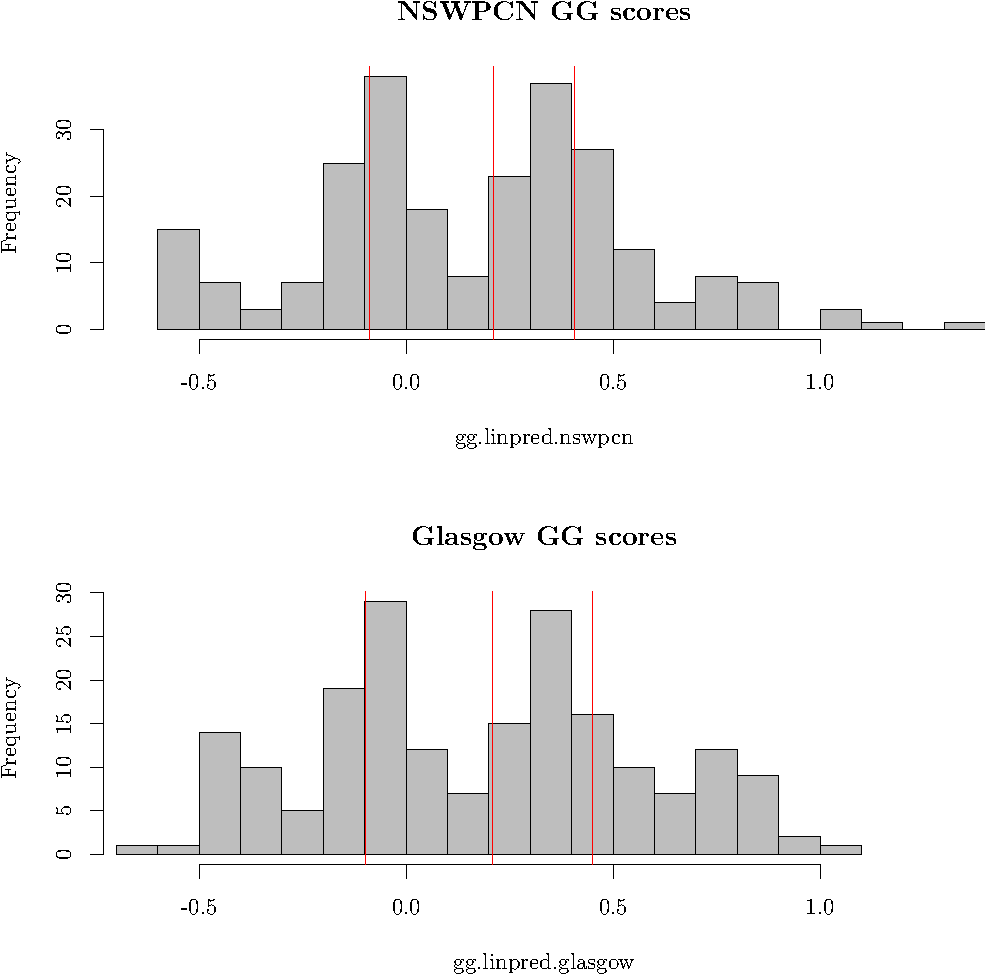
\includegraphics[width=\maxwidth]{figure/05-score-hists-1} 

}


\begin{kframe}\begin{alltt}
\hlkwd{par}\hlstd{(}\hlkwc{mfrow} \hlstd{=} \hlkwd{c}\hlstd{(}\hlnum{1}\hlstd{,} \hlnum{1}\hlstd{))}

\hlcom{# par(mfrow = c(2, 1))}
\hlcom{# hist(cph.linpred.nswpcn, main = "NSWPCN CPH scores", xlim = range(c(cph.linpred.nswpcn, cph.linpred.glasgow)), breaks = 20, col = "grey")}
\hlcom{# abline(v = quantile(gg.linpred.nswpcn, probs = c(0.25, 0.5, 0.75)), col = "red")}
\hlcom{# hist(cph.linpred.glasgow, main = "Glasgow CPH scores", xlim = range(c(cph.linpred.nswpcn, cph.linpred.glasgow)), breaks = 20, col = "grey")}
\hlcom{# abline(v = quantile(gg.linpred.glasgow, probs = c(0.25, 0.5, 0.75)), col = "red")}
\hlcom{# par(mfrow = c(1, 1))}

\hlcom{# par(mfrow = c(2, 1))}
\hlcom{# hist(rsf.linpred.nswpcn, main = "NSWPCN RSF scores", xlim = range(c(rsf.linpred.nswpcn, rsf.linpred.glasgow)), breaks = 20, col = "grey")}
\hlcom{# abline(v = quantile(rsf.linpred.nswpcn, probs = c(0.25, 0.5, 0.75)), col = "red")}
\hlcom{# hist(rsf.linpred.glasgow, main = "Glasgow RSF scores", xlim = range(c(rsf.linpred.nswpcn, rsf.linpred.glasgow)), breaks = 20, col = "grey")}
\hlcom{# abline(v = quantile(rsf.linpred.glasgow, probs = c(0.25, 0.5, 0.75)), col = "red")}
\hlcom{# par(mfrow = c(1, 1))}
\end{alltt}
\end{kframe}
\end{knitrout}

\subsection{Altman method 1 (D,F)}
\begin{knitrout}
\definecolor{shadecolor}{rgb}{0.969, 0.969, 0.969}\color{fgcolor}\begin{kframe}
\begin{alltt}
\hlkwd{summary}\hlstd{(}\hlkwd{coxph}\hlstd{(}\hlkwd{Surv}\hlstd{(Time, DSD)} \hlopt{~} \hlstd{mskcc_post.linpred.glasgow, data.glasgow))}
\end{alltt}
\begin{verbatim}
## Call:
## coxph(formula = Surv(Time, DSD) ~ mskcc_post.linpred.glasgow, 
##     data = data.glasgow)
## 
##   n= 198, number of events= 170 
## 
##                               coef exp(coef) se(coef)    z Pr(>|z|)
## mskcc_post.linpred.glasgow 0.01484   1.01495  0.00405 3.67  0.00025
## 
##                            exp(coef) exp(-coef) lower .95 upper .95
## mskcc_post.linpred.glasgow      1.01      0.985      1.01      1.02
## 
## Concordance= 0.576  (se = 0.025 )
## Rsquare= 0.067   (max possible= 0.999 )
## Likelihood ratio test= 13.6  on 1 df,   p=0.000221
## Wald test            = 13.4  on 1 df,   p=0.000245
## Score (logrank) test = 13.6  on 1 df,   p=0.000229
\end{verbatim}
\begin{alltt}
\hlkwd{summary}\hlstd{(}\hlkwd{coxph}\hlstd{(}\hlkwd{Surv}\hlstd{(Time, DSD)} \hlopt{~} \hlstd{mskcc_pre.linpred.glasgow, data.glasgow))}
\end{alltt}
\begin{verbatim}
## Call:
## coxph(formula = Surv(Time, DSD) ~ mskcc_pre.linpred.glasgow, 
##     data = data.glasgow)
## 
##   n= 198, number of events= 170 
## 
##                                coef exp(coef)  se(coef)     z Pr(>|z|)
## mskcc_pre.linpred.glasgow -0.000423  0.999577  0.007318 -0.06     0.95
## 
##                           exp(coef) exp(-coef) lower .95 upper .95
## mskcc_pre.linpred.glasgow         1          1     0.985      1.01
## 
## Concordance= 0.421  (se = 0.025 )
## Rsquare= 0   (max possible= 0.999 )
## Likelihood ratio test= 0  on 1 df,   p=0.954
## Wald test            = 0  on 1 df,   p=0.954
## Score (logrank) test = 0  on 1 df,   p=0.954
\end{verbatim}
\begin{alltt}
\hlkwd{summary}\hlstd{(}\hlkwd{coxph}\hlstd{(}\hlkwd{Surv}\hlstd{(Time, DSD)} \hlopt{~} \hlstd{gg.linpred.glasgow, data.glasgow))}
\end{alltt}
\begin{verbatim}
## Call:
## coxph(formula = Surv(Time, DSD) ~ gg.linpred.glasgow, data = data.glasgow)
## 
##   n= 198, number of events= 170 
## 
##                     coef exp(coef) se(coef)    z Pr(>|z|)
## gg.linpred.glasgow 0.746     2.109    0.221 3.38  0.00073
## 
##                    exp(coef) exp(-coef) lower .95 upper .95
## gg.linpred.glasgow      2.11      0.474      1.37      3.25
## 
## Concordance= 0.607  (se = 0.025 )
## Rsquare= 0.056   (max possible= 0.999 )
## Likelihood ratio test= 11.5  on 1 df,   p=0.000707
## Wald test            = 11.4  on 1 df,   p=0.000732
## Score (logrank) test = 11.5  on 1 df,   p=0.000693
\end{verbatim}
\begin{alltt}
\hlcom{# summary(coxph(Surv(Time, DSD) ~ cph.linpred.glasgow, data.glasgow))}
\hlcom{# summary(coxph(Surv(Time, DSD) ~ rsf.linpred.glasgow, data.glasgow))}

\hlkwd{anova}\hlstd{(}\hlkwd{coxph}\hlstd{(}\hlkwd{Surv}\hlstd{(Time, DSD)} \hlopt{~} \hlkwd{offset}\hlstd{(gg.linpred.glasgow)} \hlopt{+} \hlstd{gg.linpred.glasgow, data.glasgow))}
\end{alltt}
\begin{verbatim}
## Analysis of Deviance Table
##  Cox model: response is Surv(Time, DSD)
## Terms added sequentially (first to last)
## 
##                    loglik Chisq Df Pr(>|Chi|)
## NULL                 -724                    
## gg.linpred.glasgow   -723  1.32  1       0.25
\end{verbatim}
\begin{alltt}
\hlcom{# anova(coxph(Surv(Time, DSD) ~ offset(cph.linpred.glasgow) + cph.linpred.glasgow, data.glasgow))}
\hlcom{# anova(coxph(Surv(Time, DSD) ~ offset(rsf.linpred.glasgow) + rsf.linpred.glasgow, data.glasgow))}
\end{alltt}
\end{kframe}
\end{knitrout}
Booyah.


\subsection{Altman method 2 (F)}
\begin{knitrout}
\definecolor{shadecolor}{rgb}{0.969, 0.969, 0.969}\color{fgcolor}\begin{kframe}
\begin{alltt}
\hlkwd{summary}\hlstd{(}\hlkwd{coxph}\hlstd{(}\hlkwd{Surv}\hlstd{(Time, DSD)} \hlopt{~} \hlkwd{offset}\hlstd{(mskcc_pre.linpred.glasgow)} \hlopt{+} \hlstd{AgeCent} \hlopt{+} \hlstd{SexM} \hlopt{+} \hlstd{SizeCent} \hlopt{+} \hlstd{A2} \hlopt{+} \hlstd{A4, data.glasgow))}
\end{alltt}


{\ttfamily\noindent\color{warningcolor}{\#\# Warning in fitter(X, Y, strats, offset, init, control, weights = weights, : Ran out of iterations and did not converge}}

{\ttfamily\noindent\bfseries\color{errorcolor}{\#\# Error in fitter(X, Y, strats, offset, init, control, weights = weights, : NA/NaN/Inf in foreign function call (arg 6)}}\begin{alltt}
\hlkwd{summary}\hlstd{(}\hlkwd{coxph}\hlstd{(}\hlkwd{Surv}\hlstd{(Time, DSD)} \hlopt{~} \hlkwd{offset}\hlstd{(mskcc_post.linpred.glasgow)} \hlopt{+} \hlstd{AgeCent} \hlopt{+} \hlstd{SexM} \hlopt{+} \hlstd{SizeCent} \hlopt{+} \hlstd{A2} \hlopt{+} \hlstd{A4, data.glasgow))}
\end{alltt}
\begin{verbatim}
## Call:
## coxph(formula = Surv(Time, DSD) ~ offset(mskcc_post.linpred.glasgow) + 
##     AgeCent + SexM + SizeCent + A2 + A4, data = data.glasgow)
## 
##   n= 198, number of events= 170 
## 
##               coef exp(coef)  se(coef)      z Pr(>|z|)
## AgeCent    0.22831   1.25648   0.01006  22.69  < 2e-16
## SexMTRUE  -5.22725   0.00537   0.30189 -17.32  < 2e-16
## SizeCent   0.14973   1.16152   0.01910   7.84  4.6e-15
## A2TRUE    -2.29883   0.10038   0.37880  -6.07  1.3e-09
## A4TRUE     4.93307 138.80556   0.29941  16.48  < 2e-16
## 
##          exp(coef) exp(-coef) lower .95 upper .95
## AgeCent   1.26e+00     0.7959   1.23194    1.2815
## SexMTRUE  5.37e-03   186.2805   0.00297    0.0097
## SizeCent  1.16e+00     0.8609   1.11884    1.2058
## A2TRUE    1.00e-01     9.9625   0.04777    0.2109
## A4TRUE    1.39e+02     0.0072  77.18720  249.6137
## 
## Concordance= 0.587  (se = 0.025 )
## Rsquare= 1   (max possible= 1 )
## Likelihood ratio test= 1719  on 5 df,   p=0
## Wald test            = 2210  on 5 df,   p=0
## Score (logrank) test = 12193  on 5 df,   p=0
\end{verbatim}
\begin{alltt}
\hlkwd{summary}\hlstd{(}\hlkwd{coxph}\hlstd{(}\hlkwd{Surv}\hlstd{(Time, DSD)} \hlopt{~} \hlkwd{offset}\hlstd{(gg.linpred.glasgow)} \hlopt{+} \hlstd{AgeCent} \hlopt{+} \hlstd{SexM} \hlopt{+} \hlstd{SizeCent} \hlopt{+} \hlstd{A2} \hlopt{+} \hlstd{A4, data.glasgow))}
\end{alltt}
\begin{verbatim}
## Call:
## coxph(formula = Surv(Time, DSD) ~ offset(gg.linpred.glasgow) + 
##     AgeCent + SexM + SizeCent + A2 + A4, data = data.glasgow)
## 
##   n= 198, number of events= 170 
## 
##              coef exp(coef) se(coef)     z Pr(>|z|)
## AgeCent  -0.03255   0.96797  0.00860 -3.78  0.00015
## SexMTRUE  0.66683   1.94805  0.16160  4.13  3.7e-05
## SizeCent  0.02516   1.02547  0.00737  3.41  0.00065
## A2TRUE    0.34535   1.41249  0.17387  1.99  0.04701
## A4TRUE   -0.07127   0.93121  0.17723 -0.40  0.68757
## 
##          exp(coef) exp(-coef) lower .95 upper .95
## AgeCent      0.968      1.033     0.952     0.984
## SexMTRUE     1.948      0.513     1.419     2.674
## SizeCent     1.025      0.975     1.011     1.040
## A2TRUE       1.412      0.708     1.005     1.986
## A4TRUE       0.931      1.074     0.658     1.318
## 
## Concordance= 0.681  (se = 0.025 )
## Rsquare= 0.205   (max possible= 0.999 )
## Likelihood ratio test= 45.5  on 5 df,   p=1.12e-08
## Wald test            = 46.3  on 5 df,   p=7.74e-09
## Score (logrank) test = 48.4  on 5 df,   p=2.95e-09
\end{verbatim}
\begin{alltt}
\hlcom{# summary(coxph(Surv(Time, DSD) ~ offset(cph.linpred.glasgow) + AgeCent + SexM + SizeCent + A2 + A4, data.glasgow))}
\hlcom{# summary(coxph(Surv(Time, DSD) ~ offset(rsf.linpred.glasgow) + AgeCent + SexM + SizeCent + A2 + A4, data.glasgow))}
\end{alltt}
\end{kframe}
\end{knitrout}
Still strong evidence of misspecification or poor fit.  However, the above calibration slope was not significantly different from 1.  Hmm.  This doesn't necessarily sink the method, but will need checking as we go along.

\subsection{Altman method 3 (D)}
Look at the CIs above.

\subsection{Altman method 4 (D,C)}
\begin{knitrout}
\definecolor{shadecolor}{rgb}{0.969, 0.969, 0.969}\color{fgcolor}\begin{kframe}
\begin{alltt}
\hlstd{group_quantiles} \hlkwb{=} \hlkwd{c}\hlstd{(}\hlnum{0}\hlstd{,} \hlnum{0.25}\hlstd{,} \hlnum{0.5}\hlstd{,} \hlnum{0.75}\hlstd{,} \hlnum{1}\hlstd{)}
\hlstd{mskcc_pre.groups.glasgow} \hlkwb{=} \hlkwd{cut}\hlstd{(mskcc_pre.linpred.glasgow,} \hlkwd{quantile}\hlstd{(mskcc_pre.linpred.glasgow, group_quantiles))}
\hlstd{mskcc_post.groups.glasgow} \hlkwb{=} \hlkwd{cut}\hlstd{(mskcc_post.linpred.glasgow,} \hlkwd{quantile}\hlstd{(mskcc_post.linpred.glasgow, group_quantiles))}
\hlstd{gg.groups.glasgow} \hlkwb{=} \hlkwd{cut}\hlstd{(gg.linpred.glasgow,} \hlkwd{quantile}\hlstd{(gg.linpred.glasgow, group_quantiles))}
\hlstd{gg.groups.nswpcn} \hlkwb{=} \hlkwd{cut}\hlstd{(gg.linpred.nswpcn,} \hlkwd{quantile}\hlstd{(gg.linpred.nswpcn, group_quantiles))}
\hlstd{cph.groups.glasgow} \hlkwb{=} \hlkwd{cut}\hlstd{(cph.linpred.glasgow,} \hlkwd{quantile}\hlstd{(cph.linpred.glasgow, group_quantiles))}
\hlstd{cph.groups.nswpcn} \hlkwb{=} \hlkwd{cut}\hlstd{(cph.linpred.nswpcn,} \hlkwd{quantile}\hlstd{(cph.linpred.nswpcn, group_quantiles))}
\hlstd{rsf.groups.glasgow} \hlkwb{=} \hlkwd{cut}\hlstd{(rsf.linpred.glasgow,} \hlkwd{quantile}\hlstd{(rsf.linpred.glasgow, group_quantiles))}
\hlstd{rsf.groups.nswpcn} \hlkwb{=} \hlkwd{cut}\hlstd{(rsf.linpred.nswpcn,} \hlkwd{quantile}\hlstd{(rsf.linpred.nswpcn, group_quantiles))}

\hlkwd{par}\hlstd{(}\hlkwc{mfrow} \hlstd{=} \hlkwd{c}\hlstd{(}\hlnum{2}\hlstd{,} \hlnum{2}\hlstd{))}
\hlstd{temp} \hlkwb{=} \hlkwd{survfit}\hlstd{(}\hlkwd{Surv}\hlstd{(data.nswpcn}\hlopt{$}\hlstd{Time}\hlopt{/}\hlnum{365.25}\hlstd{, data.nswpcn}\hlopt{$}\hlstd{DSD)} \hlopt{~} \hlstd{gg.groups.nswpcn)}
\hlkwd{plot}\hlstd{(temp,} \hlkwc{col} \hlstd{= pal[}\hlnum{1}\hlopt{:}\hlstd{(}\hlkwd{length}\hlstd{(group_quantiles)}\hlopt{-}\hlnum{1}\hlstd{)],} \hlkwc{xlab} \hlstd{=} \hlstr{"Time (years)"}\hlstd{,} \hlkwc{ylab} \hlstd{=} \hlstr{"Fraction Alive"}\hlstd{,} \hlkwc{main} \hlstd{=} \hlstr{"GG: NSWPCN (Resubstitution)"}\hlstd{,} \hlkwc{xlim} \hlstd{=} \hlkwd{c}\hlstd{(}\hlnum{0}\hlstd{,} \hlnum{5}\hlstd{),} \hlkwc{lwd} \hlstd{=} \hlnum{2}\hlstd{)}
\hlkwd{legend}\hlstd{(}\hlstr{"topright"}\hlstd{,} \hlkwc{col} \hlstd{= pal[}\hlnum{1}\hlopt{:}\hlstd{(}\hlkwd{length}\hlstd{(group_quantiles)}\hlopt{-}\hlnum{1}\hlstd{)],} \hlkwc{legend} \hlstd{=} \hlkwd{gsub}\hlstd{(}\hlstr{".*="}\hlstd{,} \hlstr{""}\hlstd{,} \hlkwd{names}\hlstd{(temp}\hlopt{$}\hlstd{strata)),} \hlkwc{cex} \hlstd{=} \hlnum{0.5}\hlstd{,} \hlkwc{lwd} \hlstd{=} \hlnum{2}\hlstd{,} \hlkwc{lty} \hlstd{=} \hlstr{"solid"}\hlstd{)}

\hlstd{temp} \hlkwb{=} \hlkwd{survfit}\hlstd{(}\hlkwd{Surv}\hlstd{(data.glasgow}\hlopt{$}\hlstd{Time}\hlopt{/}\hlnum{365.25}\hlstd{, data.glasgow}\hlopt{$}\hlstd{DSD)} \hlopt{~} \hlstd{gg.groups.glasgow)}
\hlkwd{plot}\hlstd{(temp,} \hlkwc{col} \hlstd{= pal[}\hlnum{1}\hlopt{:}\hlstd{(}\hlkwd{length}\hlstd{(group_quantiles)}\hlopt{-}\hlnum{1}\hlstd{)],} \hlkwc{xlab} \hlstd{=} \hlstr{"Time (years)"}\hlstd{,} \hlkwc{ylab} \hlstd{=} \hlstr{"Fraction Alive"}\hlstd{,} \hlkwc{main} \hlstd{=} \hlstr{"GG: Glasgow"}\hlstd{,} \hlkwc{xlim} \hlstd{=} \hlkwd{c}\hlstd{(}\hlnum{0}\hlstd{,} \hlnum{5}\hlstd{),} \hlkwc{lwd} \hlstd{=} \hlnum{2}\hlstd{)}
\hlkwd{legend}\hlstd{(}\hlstr{"topright"}\hlstd{,} \hlkwc{col} \hlstd{= pal[}\hlnum{1}\hlopt{:}\hlstd{(}\hlkwd{length}\hlstd{(group_quantiles)}\hlopt{-}\hlnum{1}\hlstd{)],} \hlkwc{legend} \hlstd{=} \hlkwd{gsub}\hlstd{(}\hlstr{".*="}\hlstd{,} \hlstr{""}\hlstd{,} \hlkwd{names}\hlstd{(temp}\hlopt{$}\hlstd{strata)),} \hlkwc{cex} \hlstd{=} \hlnum{0.5}\hlstd{,} \hlkwc{lwd} \hlstd{=} \hlnum{2}\hlstd{,} \hlkwc{lty} \hlstd{=} \hlstr{"solid"}\hlstd{)}

\hlcom{# temp = survfit(Surv(data.nswpcn$Time/365.25, data.nswpcn$DSD) ~ cph.groups.nswpcn)}
\hlcom{# plot(temp, col = pal[1:(length(group_quantiles)-1)], xlab = "Time (years)", ylab = "Fraction Alive", main = "CPH: NSWPCN (Resubstitution)", xlim = c(0, 5), lwd = 2)}
\hlcom{# legend("topright", col = pal[1:(length(group_quantiles)-1)], legend = gsub(".*=", "", names(temp$strata)), cex = 0.5, lwd = 2, lty = "solid")}

\hlcom{# temp = survfit(Surv(data.glasgow$Time/365.25, data.glasgow$DSD) ~ cph.groups.glasgow)}
\hlcom{# plot(temp, col = pal[1:(length(group_quantiles)-1)], xlab = "Time (years)", ylab = "Fraction Alive", main = "CPH: Glasgow", xlim = c(0, 5), lwd = 2)}
\hlcom{# legend("topright", col = pal[1:(length(group_quantiles)-1)], legend = gsub(".*=", "", names(temp$strata)), cex = 0.5, lwd = 2, lty = "solid")}

\hlcom{# temp = survfit(Surv(data.nswpcn$Time/365.25, data.nswpcn$DSD) ~ rsf.groups.nswpcn)}
\hlcom{# plot(temp, col = pal[1:(length(group_quantiles)-1)], xlab = "Time (years)", ylab = "Fraction Alive", main = "RSF: NSWPCN (Resubstitution)", xlim = c(0, 5), lwd = 2)}
\hlcom{# legend("topright", col = pal[1:(length(group_quantiles)-1)], legend = gsub(".*=", "", names(temp$strata)), cex = 0.5, lwd = 2, lty = "solid")}

\hlcom{# temp = survfit(Surv(data.glasgow$Time/365.25, data.glasgow$DSD) ~ rsf.groups.glasgow)}
\hlcom{# plot(temp, col = pal[1:(length(group_quantiles)-1)], xlab = "Time (years)", ylab = "Fraction Alive", main = "RSF: Glasgow", xlim = c(0, 5), lwd = 2)}
\hlcom{# legend("topright", col = pal[1:(length(group_quantiles)-1)], legend = gsub(".*=", "", names(temp$strata)), cex = 0.5, lwd = 2, lty = "solid")}

\hlstd{temp} \hlkwb{=} \hlkwd{survfit}\hlstd{(}\hlkwd{Surv}\hlstd{(data.glasgow}\hlopt{$}\hlstd{Time}\hlopt{/}\hlnum{365.25}\hlstd{, data.glasgow}\hlopt{$}\hlstd{DSD)} \hlopt{~} \hlstd{mskcc_pre.groups.glasgow)}
\hlkwd{plot}\hlstd{(temp,} \hlkwc{col} \hlstd{= pal[}\hlnum{1}\hlopt{:}\hlstd{(}\hlkwd{length}\hlstd{(group_quantiles)}\hlopt{-}\hlnum{1}\hlstd{)],} \hlkwc{xlab} \hlstd{=} \hlstr{"Time (years)"}\hlstd{,} \hlkwc{ylab} \hlstd{=} \hlstr{"Fraction Alive"}\hlstd{,} \hlkwc{main} \hlstd{=} \hlstr{"MSKCC Preop: Glasgow"}\hlstd{,} \hlkwc{xlim} \hlstd{=} \hlkwd{c}\hlstd{(}\hlnum{0}\hlstd{,} \hlnum{5}\hlstd{),} \hlkwc{lwd} \hlstd{=} \hlnum{2}\hlstd{)}
\hlkwd{legend}\hlstd{(}\hlstr{"topright"}\hlstd{,} \hlkwc{col} \hlstd{= pal[}\hlnum{1}\hlopt{:}\hlstd{(}\hlkwd{length}\hlstd{(group_quantiles)}\hlopt{-}\hlnum{1}\hlstd{)],} \hlkwc{legend} \hlstd{=} \hlkwd{gsub}\hlstd{(}\hlstr{".*="}\hlstd{,} \hlstr{""}\hlstd{,} \hlkwd{names}\hlstd{(temp}\hlopt{$}\hlstd{strata)),} \hlkwc{cex} \hlstd{=} \hlnum{0.5}\hlstd{,} \hlkwc{lwd} \hlstd{=} \hlnum{2}\hlstd{,} \hlkwc{lty} \hlstd{=} \hlstr{"solid"}\hlstd{)}

\hlstd{temp} \hlkwb{=} \hlkwd{survfit}\hlstd{(}\hlkwd{Surv}\hlstd{(data.glasgow}\hlopt{$}\hlstd{Time}\hlopt{/}\hlnum{365.25}\hlstd{, data.glasgow}\hlopt{$}\hlstd{DSD)} \hlopt{~} \hlstd{mskcc_post.groups.glasgow)}
\hlkwd{plot}\hlstd{(temp,} \hlkwc{col} \hlstd{= pal[}\hlnum{1}\hlopt{:}\hlstd{(}\hlkwd{length}\hlstd{(group_quantiles)}\hlopt{-}\hlnum{1}\hlstd{)],} \hlkwc{xlab} \hlstd{=} \hlstr{"Time (years)"}\hlstd{,} \hlkwc{ylab} \hlstd{=} \hlstr{"Fraction Alive"}\hlstd{,} \hlkwc{main} \hlstd{=} \hlstr{"MSKCC Postop: Glasgow"}\hlstd{,} \hlkwc{xlim} \hlstd{=} \hlkwd{c}\hlstd{(}\hlnum{0}\hlstd{,} \hlnum{5}\hlstd{),} \hlkwc{lwd} \hlstd{=} \hlnum{2}\hlstd{)}
\hlkwd{legend}\hlstd{(}\hlstr{"topright"}\hlstd{,} \hlkwc{col} \hlstd{= pal[}\hlnum{1}\hlopt{:}\hlstd{(}\hlkwd{length}\hlstd{(group_quantiles)}\hlopt{-}\hlnum{1}\hlstd{)],} \hlkwc{legend} \hlstd{=} \hlkwd{gsub}\hlstd{(}\hlstr{".*="}\hlstd{,} \hlstr{""}\hlstd{,} \hlkwd{names}\hlstd{(temp}\hlopt{$}\hlstd{strata)),} \hlkwc{cex} \hlstd{=} \hlnum{0.5}\hlstd{,} \hlkwc{lwd} \hlstd{=} \hlnum{2}\hlstd{,} \hlkwc{lty} \hlstd{=} \hlstr{"solid"}\hlstd{)}
\end{alltt}
\end{kframe}

{\centering 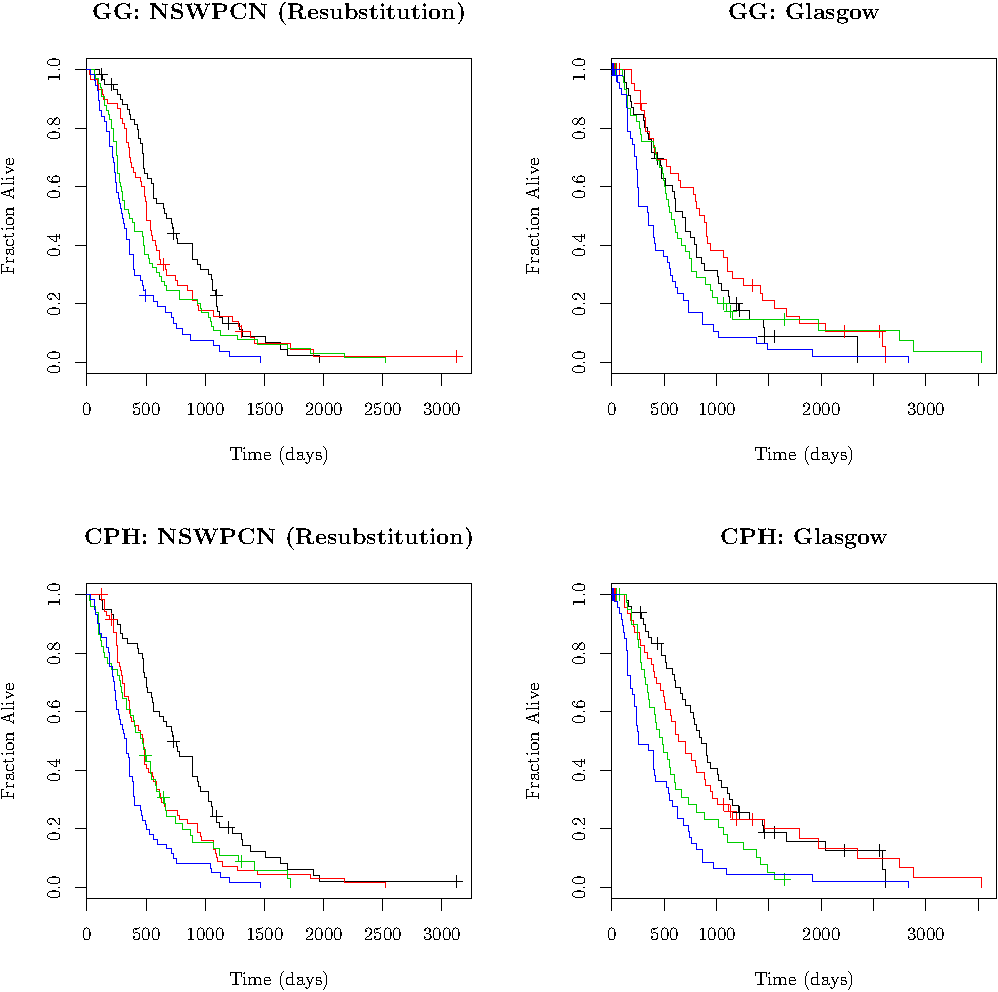
\includegraphics[width=\maxwidth]{figure/05-altman-4-1} 

}


\begin{kframe}\begin{alltt}
\hlkwd{par}\hlstd{(}\hlkwc{mfrow} \hlstd{=} \hlkwd{c}\hlstd{(}\hlnum{1}\hlstd{,} \hlnum{1}\hlstd{))}
\end{alltt}
\end{kframe}
\end{knitrout}
Weird.  MSKCC somehow is still finding a subgroup, and it's somehow even clearer in preop!  This is based on an approximation to GG only, but should be pretty close.  It certainly does OK on resubstituted data, but not so well on the Glasgow patients.


Decision curve analysis.
\begin{knitrout}
\definecolor{shadecolor}{rgb}{0.969, 0.969, 0.969}\color{fgcolor}\begin{kframe}
\begin{alltt}
\hlkwd{source}\hlstd{(}\hlstr{"stdca.R"}\hlstd{)}
\hlstd{temp.data} \hlkwb{=} \hlkwd{data.frame}\hlstd{(}\hlkwc{Time} \hlstd{= data.glasgow}\hlopt{$}\hlstd{Time,} \hlkwc{DSD} \hlstd{= data.glasgow}\hlopt{$}\hlstd{DSD}\hlopt{*}\hlnum{1}\hlstd{,}
    \hlkwc{gg.1} \hlstd{=} \hlnum{1}\hlopt{-}\hlstd{gg.prob.glasgow[val.prob.times} \hlopt{==} \hlnum{365}\hlstd{,],} \hlkwc{gg.2} \hlstd{=} \hlnum{1}\hlopt{-}\hlstd{gg.prob.glasgow[val.prob.times} \hlopt{==} \hlnum{365}\hlopt{*}\hlnum{2}\hlstd{,],} \hlkwc{gg.3} \hlstd{=} \hlnum{1}\hlopt{-}\hlstd{gg.prob.glasgow[val.prob.times} \hlopt{==} \hlnum{365}\hlopt{*}\hlnum{3}\hlstd{,],}
    \hlkwc{cph.1} \hlstd{=} \hlnum{1}\hlopt{-}\hlstd{cph.prob.glasgow[val.prob.times} \hlopt{==} \hlnum{365}\hlstd{,],} \hlkwc{cph.2} \hlstd{=} \hlnum{1}\hlopt{-}\hlstd{cph.prob.glasgow[val.prob.times} \hlopt{==} \hlnum{365}\hlopt{*}\hlnum{2}\hlstd{,],} \hlkwc{cph.3} \hlstd{=} \hlnum{1}\hlopt{-}\hlstd{cph.prob.glasgow[val.prob.times} \hlopt{==} \hlnum{365}\hlopt{*}\hlnum{3}\hlstd{,],}
    \hlkwc{rsf.1} \hlstd{=} \hlnum{1}\hlopt{-}\hlstd{rsf.prob.glasgow[val.prob.times} \hlopt{==} \hlnum{365}\hlstd{,],} \hlkwc{rsf.2} \hlstd{=} \hlnum{1}\hlopt{-}\hlstd{rsf.prob.glasgow[val.prob.times} \hlopt{==} \hlnum{365}\hlopt{*}\hlnum{2}\hlstd{,],} \hlkwc{rsf.3} \hlstd{=} \hlnum{1}\hlopt{-}\hlstd{rsf.prob.glasgow[val.prob.times} \hlopt{==} \hlnum{365}\hlopt{*}\hlnum{3}\hlstd{,],}
    \hlkwc{mskcc.pre.1} \hlstd{=} \hlnum{1}\hlopt{-}\hlstd{mskcc_pre.12mo.glasgow,} \hlkwc{mskcc.pre.2} \hlstd{=} \hlnum{1}\hlopt{-}\hlstd{mskcc_pre.24mo.glasgow,} \hlkwc{mskcc.pre.3} \hlstd{=} \hlnum{1}\hlopt{-}\hlstd{mskcc_pre.36mo.glasgow,}
    \hlkwc{mskcc.post.1} \hlstd{=} \hlnum{1}\hlopt{-}\hlstd{mskcc_post.12mo.glasgow,} \hlkwc{mskcc.post.2} \hlstd{=} \hlnum{1}\hlopt{-}\hlstd{mskcc_post.24mo.glasgow,} \hlkwc{mskcc.post.3} \hlstd{=} \hlnum{1}\hlopt{-}\hlstd{mskcc_post.36mo.glasgow)}
\hlcom{# invisible(stdca(data = temp.data, outcome = "DSD", ttoutcome = "Time", predictors = c("gg.1", "cph.1", "rsf.1", "mskcc.pre.1", "mskcc.post.1"), timepoint = 365, probability = rep(TRUE, 5)))}
\hlcom{# invisible(stdca(data = temp.data, outcome = "DSD", ttoutcome = "Time", predictors = c("gg.2", "cph.2", "rsf.2", "mskcc.pre.2", "mskcc.post.2"), timepoint = 365*2, probability = rep(TRUE, 5)))}
\hlcom{# invisible(stdca(data = temp.data, outcome = "DSD", ttoutcome = "Time", predictors = c("gg.3", "cph.3", "rsf.3", "mskcc.pre.3", "mskcc.post.3"), timepoint = 365*3, probability = rep(TRUE, 5)))}
\hlkwd{invisible}\hlstd{(}\hlkwd{stdca}\hlstd{(}\hlkwc{data} \hlstd{= temp.data,} \hlkwc{outcome} \hlstd{=} \hlstr{"DSD"}\hlstd{,} \hlkwc{ttoutcome} \hlstd{=} \hlstr{"Time"}\hlstd{,} \hlkwc{predictors} \hlstd{=} \hlkwd{c}\hlstd{(}\hlstr{"gg.1"}\hlstd{,} \hlstr{"mskcc.pre.1"}\hlstd{,} \hlstr{"mskcc.post.1"}\hlstd{),} \hlkwc{timepoint} \hlstd{=} \hlnum{365}\hlstd{,} \hlkwc{probability} \hlstd{=} \hlkwd{rep}\hlstd{(}\hlnum{TRUE}\hlstd{,} \hlnum{5}\hlstd{)))}
\end{alltt}


{\ttfamily\noindent\bfseries\color{errorcolor}{\#\# Error in stdca(data = temp.data, outcome = "{}DSD"{}, ttoutcome = "{}Time"{}, : Number of probabilities specified must be the same as the number of predictors being checked.}}\begin{alltt}
\hlkwd{invisible}\hlstd{(}\hlkwd{stdca}\hlstd{(}\hlkwc{data} \hlstd{= temp.data,} \hlkwc{outcome} \hlstd{=} \hlstr{"DSD"}\hlstd{,} \hlkwc{ttoutcome} \hlstd{=} \hlstr{"Time"}\hlstd{,} \hlkwc{predictors} \hlstd{=} \hlkwd{c}\hlstd{(}\hlstr{"gg.2"}\hlstd{,} \hlstr{"mskcc.pre.2"}\hlstd{,} \hlstr{"mskcc.post.2"}\hlstd{),} \hlkwc{timepoint} \hlstd{=} \hlnum{365}\hlopt{*}\hlnum{2}\hlstd{,} \hlkwc{probability} \hlstd{=} \hlkwd{rep}\hlstd{(}\hlnum{TRUE}\hlstd{,} \hlnum{5}\hlstd{)))}
\end{alltt}


{\ttfamily\noindent\bfseries\color{errorcolor}{\#\# Error in stdca(data = temp.data, outcome = "{}DSD"{}, ttoutcome = "{}Time"{}, : Number of probabilities specified must be the same as the number of predictors being checked.}}\begin{alltt}
\hlkwd{invisible}\hlstd{(}\hlkwd{stdca}\hlstd{(}\hlkwc{data} \hlstd{= temp.data,} \hlkwc{outcome} \hlstd{=} \hlstr{"DSD"}\hlstd{,} \hlkwc{ttoutcome} \hlstd{=} \hlstr{"Time"}\hlstd{,} \hlkwc{predictors} \hlstd{=} \hlkwd{c}\hlstd{(}\hlstr{"gg.3"}\hlstd{,} \hlstr{"mskcc.pre.3"}\hlstd{,} \hlstr{"mskcc.post.3"}\hlstd{),} \hlkwc{timepoint} \hlstd{=} \hlnum{365}\hlopt{*}\hlnum{3}\hlstd{,} \hlkwc{probability} \hlstd{=} \hlkwd{rep}\hlstd{(}\hlnum{TRUE}\hlstd{,} \hlnum{5}\hlstd{)))}
\end{alltt}


{\ttfamily\noindent\bfseries\color{errorcolor}{\#\# Error in stdca(data = temp.data, outcome = "{}DSD"{}, ttoutcome = "{}Time"{}, : Number of probabilities specified must be the same as the number of predictors being checked.}}\end{kframe}
\end{knitrout}


\subsection{Brier score}
\begin{knitrout}
\definecolor{shadecolor}{rgb}{0.969, 0.969, 0.969}\color{fgcolor}\begin{kframe}
\begin{alltt}
\hlstd{calcIBS} \hlkwb{=} \hlkwa{function}\hlstd{(}\hlkwc{surv}\hlstd{,} \hlkwc{pred}\hlstd{,} \hlkwc{pred_times}\hlstd{,} \hlkwc{max_time}\hlstd{,} \hlkwc{min_time} \hlstd{=} \hlnum{0}\hlstd{)}
\hlstd{\{}
        \hlkwd{stopifnot}\hlstd{(}\hlkwd{nrow}\hlstd{(surv)} \hlopt{==} \hlkwd{nrow}\hlstd{(pred)} \hlopt{&&} \hlkwd{length}\hlstd{(pred_times)} \hlopt{==} \hlkwd{ncol}\hlstd{(pred))}

        \hlstd{n} \hlkwb{=} \hlkwd{nrow}\hlstd{(surv)}
        \hlstd{marg_survfit} \hlkwb{=} \hlkwd{survfit}\hlstd{(surv} \hlopt{~} \hlnum{1}\hlstd{)}
        \hlstd{marg_censfit} \hlkwb{=} \hlkwd{survfit}\hlstd{(}\hlkwd{Surv}\hlstd{(surv[,}\hlnum{1}\hlstd{],} \hlopt{!}\hlstd{surv[,}\hlnum{2}\hlstd{])} \hlopt{~} \hlnum{1}\hlstd{)}
        \hlstd{marg_surv_func} \hlkwb{=} \hlkwd{approxfun}\hlstd{(marg_survfit}\hlopt{$}\hlstd{time, marg_survfit}\hlopt{$}\hlstd{surv,} \hlkwc{method} \hlstd{=} \hlstr{"constant"}\hlstd{,} \hlkwc{yleft} \hlstd{=} \hlnum{1}\hlstd{,} \hlkwc{yright} \hlstd{=} \hlnum{0}\hlstd{,} \hlkwc{rule} \hlstd{=} \hlnum{2}\hlopt{:}\hlnum{1}\hlstd{,} \hlkwc{f} \hlstd{=} \hlnum{0}\hlstd{)}
        \hlstd{marg_cens_func} \hlkwb{=} \hlkwd{approxfun}\hlstd{(marg_censfit}\hlopt{$}\hlstd{time, marg_censfit}\hlopt{$}\hlstd{surv,} \hlkwc{method} \hlstd{=} \hlstr{"constant"}\hlstd{,} \hlkwc{yleft} \hlstd{=} \hlnum{1}\hlstd{,} \hlkwc{yright} \hlstd{=} \hlnum{0}\hlstd{,} \hlkwc{rule} \hlstd{=} \hlnum{2}\hlopt{:}\hlnum{1}\hlstd{,} \hlkwc{f} \hlstd{=} \hlnum{0}\hlstd{)}

        \hlstd{pred_funcs} \hlkwb{=} \hlkwd{apply}\hlstd{(pred,} \hlnum{1}\hlstd{,} \hlkwa{function}\hlstd{(}\hlkwc{pat_preds}\hlstd{)} \hlkwd{approxfun}\hlstd{(pred_times, pat_preds,} \hlkwc{yleft} \hlstd{=} \hlnum{1}\hlstd{,} \hlkwc{yright} \hlstd{=} \hlkwd{min}\hlstd{(pat_preds),} \hlkwc{rule} \hlstd{=} \hlnum{2}\hlstd{))}

        \hlstd{indiv_patient_bsc} \hlkwb{=} \hlkwa{function}\hlstd{(}\hlkwc{pat_i}\hlstd{,} \hlkwc{tstars}\hlstd{)}
        \hlstd{\{}
                \hlstd{observed_time} \hlkwb{=} \hlstd{surv[pat_i,} \hlnum{1}\hlstd{]}
                \hlstd{observed_event} \hlkwb{=} \hlstd{surv[pat_i,} \hlnum{2}\hlstd{]}
                \hlstd{pred_func} \hlkwb{=} \hlstd{pred_funcs[[pat_i]]}
                \hlstd{category} \hlkwb{=} \hlnum{1}\hlopt{*}\hlstd{(observed_time} \hlopt{<=} \hlstd{tstars} \hlopt{&} \hlstd{observed_event)} \hlopt{+} \hlnum{2}\hlopt{*}\hlstd{(observed_time} \hlopt{>} \hlstd{tstars)} \hlopt{+} \hlnum{3}\hlopt{*}\hlstd{(observed_time} \hlopt{<=} \hlstd{tstars} \hlopt{& !}\hlstd{observed_event)}
                \hlstd{bsc} \hlkwb{=} \hlkwd{rep}\hlstd{(}\hlnum{NA}\hlstd{,} \hlkwd{length}\hlstd{(tstars))}
                \hlstd{bsc[category} \hlopt{==} \hlnum{1}\hlstd{]} \hlkwb{=} \hlkwd{pred_func}\hlstd{(tstars[category} \hlopt{==} \hlnum{1}\hlstd{])}\hlopt{^}\hlnum{2} \hlopt{/} \hlkwd{marg_cens_func}\hlstd{(observed_time)}
                \hlstd{bsc[category} \hlopt{==} \hlnum{2}\hlstd{]} \hlkwb{=} \hlstd{(}\hlnum{1} \hlopt{-} \hlkwd{pred_func}\hlstd{(tstars[category} \hlopt{==} \hlnum{2}\hlstd{]))}\hlopt{^}\hlnum{2} \hlopt{/} \hlkwd{marg_cens_func}\hlstd{(tstars[category} \hlopt{==} \hlnum{2}\hlstd{])}
                \hlstd{bsc[category} \hlopt{==} \hlnum{3}\hlstd{]} \hlkwb{=} \hlnum{0}
                \hlstd{bsc}
        \hlstd{\}}

        \hlstd{bsc_func} \hlkwb{=} \hlkwa{function}\hlstd{(}\hlkwc{tstars}\hlstd{) \{} \hlkwd{rowMeans}\hlstd{(}\hlkwd{sapply}\hlstd{(}\hlnum{1}\hlopt{:}\hlstd{n,} \hlkwa{function}\hlstd{(}\hlkwc{pat_i}\hlstd{)} \hlkwd{indiv_patient_bsc}\hlstd{(pat_i, tstars))) \}}

        \hlstd{weight_func} \hlkwb{=} \hlkwa{function}\hlstd{(}\hlkwc{tstars}\hlstd{) \{ (}\hlnum{1} \hlopt{-} \hlkwd{marg_surv_func}\hlstd{(tstars))} \hlopt{/} \hlstd{(}\hlnum{1} \hlopt{-} \hlkwd{marg_surv_func}\hlstd{(max_time)) \}}

        \hlcom{# Be slack and do trapezoidal int. with a fine grid.  It should be possible }
        \hlcom{# to calulate the int. exactly but I cbfed.}
        \hlstd{int_grid} \hlkwb{=} \hlkwd{seq}\hlstd{(min_time, max_time,} \hlkwc{length.out} \hlstd{=} \hlnum{1e3}\hlstd{)}
        \hlstd{bsc_vals} \hlkwb{=} \hlkwd{bsc_func}\hlstd{(int_grid)}
        \hlstd{weight_vals} \hlkwb{=} \hlkwd{weight_func}\hlstd{(int_grid)}
        \hlstd{int_vals} \hlkwb{=} \hlstd{bsc_vals} \hlopt{*} \hlstd{weight_vals}
        \hlstd{ibsc} \hlkwb{=} \hlstd{(}\hlnum{2}\hlopt{*}\hlkwd{sum}\hlstd{(int_vals)} \hlopt{-} \hlstd{int_vals[}\hlnum{1}\hlstd{]} \hlopt{-} \hlstd{int_vals[}\hlkwd{length}\hlstd{(int_vals)])} \hlopt{*} \hlstd{(}\hlkwd{diff}\hlstd{(}\hlkwd{range}\hlstd{(int_grid)))} \hlopt{/} \hlstd{(}\hlnum{2}\hlopt{*}\hlkwd{length}\hlstd{(int_vals))}

        \hlkwd{return}\hlstd{(}\hlkwd{list}\hlstd{(}\hlkwc{bsc} \hlstd{= bsc_vals,} \hlkwc{weights} \hlstd{= weight_vals,} \hlkwc{eval_times} \hlstd{= int_grid,} \hlkwc{ibsc} \hlstd{= ibsc))}
\hlstd{\}}

\hlstd{calcBSsingle} \hlkwb{=} \hlkwa{function}\hlstd{(}\hlkwc{surv}\hlstd{,} \hlkwc{pred}\hlstd{,} \hlkwc{pred_time}\hlstd{)}
\hlstd{\{}
        \hlstd{n} \hlkwb{=} \hlkwd{nrow}\hlstd{(surv)}
        \hlstd{obs_time} \hlkwb{=} \hlstd{surv[,}\hlnum{1}\hlstd{]}
        \hlstd{obs_event} \hlkwb{=} \hlstd{surv[,}\hlnum{2}\hlstd{]}
        \hlstd{marg_censfit} \hlkwb{=} \hlkwd{survfit}\hlstd{(}\hlkwd{Surv}\hlstd{(obs_time,} \hlopt{!}\hlstd{obs_event)} \hlopt{~} \hlnum{1}\hlstd{)}
        \hlstd{marg_cens_func} \hlkwb{=} \hlkwd{approxfun}\hlstd{(marg_censfit}\hlopt{$}\hlstd{time, marg_censfit}\hlopt{$}\hlstd{surv,} \hlkwc{method} \hlstd{=} \hlstr{"constant"}\hlstd{,} \hlkwc{yleft} \hlstd{=} \hlnum{1}\hlstd{,} \hlkwc{yright} \hlstd{=} \hlnum{0}\hlstd{,} \hlkwc{rule} \hlstd{=} \hlnum{2}\hlopt{:}\hlnum{1}\hlstd{,} \hlkwc{f} \hlstd{=} \hlnum{0}\hlstd{)}

        \hlstd{brier_val} \hlkwb{=} \hlkwd{rep}\hlstd{(}\hlnum{NA}\hlstd{, n)}
        \hlstd{cat} \hlkwb{=} \hlnum{1}\hlopt{*}\hlkwd{I}\hlstd{(obs_time} \hlopt{<=} \hlstd{pred_time} \hlopt{&} \hlstd{obs_event)} \hlopt{+} \hlnum{2}\hlopt{*}\hlkwd{I}\hlstd{(obs_time} \hlopt{>} \hlstd{pred_time)} \hlopt{+} \hlnum{3}\hlopt{*}\hlkwd{I}\hlstd{(obs_time} \hlopt{<=} \hlstd{pred_time} \hlopt{& !}\hlstd{obs_event)}
        \hlstd{brier_val[cat} \hlopt{==} \hlnum{1}\hlstd{]} \hlkwb{=} \hlstd{(pred[cat} \hlopt{==} \hlnum{1}\hlstd{])}\hlopt{^}\hlnum{2} \hlopt{/} \hlkwd{marg_cens_func}\hlstd{(obs_time[cat} \hlopt{==} \hlnum{1}\hlstd{])}
        \hlstd{brier_val[cat} \hlopt{==} \hlnum{2}\hlstd{]} \hlkwb{=} \hlstd{(}\hlnum{1}\hlopt{-}\hlstd{pred[cat} \hlopt{==} \hlnum{2}\hlstd{])}\hlopt{^}\hlnum{2} \hlopt{/} \hlkwd{marg_cens_func}\hlstd{(pred_time)}
        \hlstd{brier_val[cat} \hlopt{==} \hlnum{3}\hlstd{]} \hlkwb{=} \hlnum{0}

        \hlkwd{mean}\hlstd{(brier_val)}
\hlstd{\}}
\end{alltt}
\end{kframe}
\end{knitrout}


\begin{knitrout}
\definecolor{shadecolor}{rgb}{0.969, 0.969, 0.969}\color{fgcolor}\begin{kframe}
\begin{alltt}
\hlstd{mskcc_post.12mo.glasgow.brier} \hlkwb{=} \hlkwd{calcBSsingle}\hlstd{(}\hlkwd{Surv}\hlstd{(data.glasgow}\hlopt{$}\hlstd{Time, data.glasgow}\hlopt{$}\hlstd{DSD), mskcc_post.12mo.glasgow,} \hlnum{12}\hlopt{/}\hlnum{12}\hlopt{*}\hlnum{365.25}\hlstd{)}
\hlstd{mskcc_post.24mo.glasgow.brier} \hlkwb{=} \hlkwd{calcBSsingle}\hlstd{(}\hlkwd{Surv}\hlstd{(data.glasgow}\hlopt{$}\hlstd{Time, data.glasgow}\hlopt{$}\hlstd{DSD), mskcc_post.24mo.glasgow,} \hlnum{24}\hlopt{/}\hlnum{12}\hlopt{*}\hlnum{365.25}\hlstd{)}
\hlstd{mskcc_post.36mo.glasgow.brier} \hlkwb{=} \hlkwd{calcBSsingle}\hlstd{(}\hlkwd{Surv}\hlstd{(data.glasgow}\hlopt{$}\hlstd{Time, data.glasgow}\hlopt{$}\hlstd{DSD), mskcc_post.36mo.glasgow,} \hlnum{36}\hlopt{/}\hlnum{12}\hlopt{*}\hlnum{365.25}\hlstd{)}
\hlstd{mskcc_pre.12mo.glasgow.brier} \hlkwb{=} \hlkwd{calcBSsingle}\hlstd{(}\hlkwd{Surv}\hlstd{(data.glasgow}\hlopt{$}\hlstd{Time, data.glasgow}\hlopt{$}\hlstd{DSD), mskcc_pre.12mo.glasgow,} \hlnum{12}\hlopt{/}\hlnum{12}\hlopt{*}\hlnum{365.25}\hlstd{)}
\hlstd{mskcc_pre.24mo.glasgow.brier} \hlkwb{=} \hlkwd{calcBSsingle}\hlstd{(}\hlkwd{Surv}\hlstd{(data.glasgow}\hlopt{$}\hlstd{Time, data.glasgow}\hlopt{$}\hlstd{DSD), mskcc_pre.24mo.glasgow,} \hlnum{24}\hlopt{/}\hlnum{12}\hlopt{*}\hlnum{365.25}\hlstd{)}
\hlstd{mskcc_pre.36mo.glasgow.brier} \hlkwb{=} \hlkwd{calcBSsingle}\hlstd{(}\hlkwd{Surv}\hlstd{(data.glasgow}\hlopt{$}\hlstd{Time, data.glasgow}\hlopt{$}\hlstd{DSD), mskcc_pre.36mo.glasgow,} \hlnum{36}\hlopt{/}\hlnum{12}\hlopt{*}\hlnum{365.25}\hlstd{)}
\hlstd{gg.path.glasgow.brier} \hlkwb{=} \hlkwd{calcIBS}\hlstd{(}\hlkwd{Surv}\hlstd{(data.glasgow}\hlopt{$}\hlstd{Time, data.glasgow}\hlopt{$}\hlstd{DSD),} \hlkwd{t}\hlstd{(}\hlkwd{sapply}\hlstd{(gg.path.glasgow,} \hlkwa{function}\hlstd{(}\hlkwc{x}\hlstd{) x[,}\hlnum{2}\hlstd{])), gg.path.glasgow[[}\hlnum{1}\hlstd{]][,}\hlnum{1}\hlstd{],} \hlnum{10}\hlopt{*}\hlnum{365.25}\hlstd{)}

\hlstd{km0.path.glasgow.brier} \hlkwb{=} \hlkwd{calcIBS}\hlstd{(}\hlkwd{Surv}\hlstd{(data.glasgow}\hlopt{$}\hlstd{Time, data.glasgow}\hlopt{$}\hlstd{DSD),} \hlkwd{matrix}\hlstd{(fit.km0}\hlopt{$}\hlstd{surv,} \hlkwc{nrow} \hlstd{=} \hlkwd{nrow}\hlstd{(data.glasgow),} \hlkwc{ncol} \hlstd{=} \hlkwd{length}\hlstd{(fit.km0}\hlopt{$}\hlstd{time),} \hlkwc{byrow} \hlstd{=} \hlnum{TRUE}\hlstd{), fit.km0}\hlopt{$}\hlstd{time,} \hlnum{10}\hlopt{*}\hlnum{365.25}\hlstd{)}

\hlstd{temp.cph.pred} \hlkwb{=} \hlkwd{survfit}\hlstd{(fit.cph,} \hlkwc{newdata} \hlstd{= data.glasgow)}
\hlstd{temp.cph.pred.expanded_strata} \hlkwb{=} \hlkwd{rep}\hlstd{(}\hlkwd{names}\hlstd{(temp.cph.pred}\hlopt{$}\hlstd{strata), temp.cph.pred}\hlopt{$}\hlstd{strata)}
\hlstd{temp.cph.pred_funcs} \hlkwb{=} \hlkwd{sapply}\hlstd{(}\hlkwd{rownames}\hlstd{(data.glasgow),} \hlkwa{function}\hlstd{(}\hlkwc{pat_id}\hlstd{) \{}
        \hlkwd{approxfun}\hlstd{(temp.cph.pred}\hlopt{$}\hlstd{time[temp.cph.pred.expanded_strata} \hlopt{==} \hlstd{pat_id], temp.cph.pred}\hlopt{$}\hlstd{surv[temp.cph.pred.expanded_strata} \hlopt{==} \hlstd{pat_id],} \hlkwc{method} \hlstd{=} \hlstr{"constant"}\hlstd{,} \hlkwc{f} \hlstd{=} \hlnum{0}\hlstd{,} \hlkwc{yleft} \hlstd{=} \hlnum{1}\hlstd{,} \hlkwc{rule} \hlstd{=} \hlnum{2}\hlstd{)}
\hlstd{\})}
\hlstd{temp.brier.times} \hlkwb{=} \hlkwd{unique}\hlstd{(}\hlkwd{sort}\hlstd{(}\hlkwd{c}\hlstd{(}\hlkwd{seq}\hlstd{(}\hlnum{0}\hlstd{,} \hlnum{10}\hlopt{*}\hlnum{365.25}\hlstd{,} \hlnum{1}\hlstd{),} \hlkwd{c}\hlstd{(}\hlnum{12}\hlstd{,} \hlnum{24}\hlstd{,} \hlnum{36}\hlstd{)}\hlopt{/}\hlnum{12}\hlopt{*}\hlnum{365.25}\hlstd{)))}
\hlstd{cph.path.glasgow.brier} \hlkwb{=} \hlkwd{calcIBS}\hlstd{(}\hlkwd{Surv}\hlstd{(data.glasgow}\hlopt{$}\hlstd{Time, data.glasgow}\hlopt{$}\hlstd{DSD),}
        \hlkwd{t}\hlstd{(}\hlkwd{sapply}\hlstd{(temp.cph.pred_funcs[}\hlkwd{rownames}\hlstd{(data.glasgow)],} \hlkwa{function}\hlstd{(}\hlkwc{f}\hlstd{)} \hlkwd{f}\hlstd{(temp.brier.times))), temp.brier.times,} \hlnum{10}\hlopt{*}\hlnum{365.25}\hlstd{)}

\hlstd{temp.rsf.pred} \hlkwb{=} \hlkwd{predict}\hlstd{(fit.rsf,} \hlkwc{newdata} \hlstd{= data.glasgow)}
\hlstd{rsf.path.glasgow.brier} \hlkwb{=} \hlkwd{calcIBS}\hlstd{(}\hlkwd{Surv}\hlstd{(data.glasgow}\hlopt{$}\hlstd{Time, data.glasgow}\hlopt{$}\hlstd{DSD),} \hlkwd{t}\hlstd{(}\hlkwd{apply}\hlstd{(temp.rsf.pred}\hlopt{$}\hlstd{survival,} \hlnum{1}\hlstd{,} \hlkwa{function}\hlstd{(}\hlkwc{patpreds}\hlstd{)} \hlkwd{approx}\hlstd{(temp.rsf.pred}\hlopt{$}\hlstd{time.interest, patpreds, temp.brier.times)}\hlopt{$}\hlstd{y)), temp.brier.times,} \hlnum{10}\hlopt{*}\hlnum{365.25}\hlstd{)}
\end{alltt}
\end{kframe}
\end{knitrout}

\begin{knitrout}
\definecolor{shadecolor}{rgb}{0.969, 0.969, 0.969}\color{fgcolor}\begin{kframe}
\begin{alltt}
\hlkwd{plot}\hlstd{(gg.path.glasgow.brier}\hlopt{$}\hlstd{eval_times}\hlopt{/}\hlnum{365.25}\hlopt{*}\hlnum{12}\hlstd{, gg.path.glasgow.brier}\hlopt{$}\hlstd{bsc,} \hlkwc{col} \hlstd{= pal[}\hlstr{"gg"}\hlstd{],} \hlkwc{type} \hlstd{=} \hlstr{"l"}\hlstd{,} \hlkwc{ylim} \hlstd{=} \hlkwd{c}\hlstd{(}\hlnum{0}\hlstd{,} \hlnum{0.3}\hlstd{),} \hlkwc{xlab} \hlstd{=} \hlstr{"Time from diagnosis (months)"}\hlstd{,} \hlkwc{ylab} \hlstd{=} \hlstr{"Brier score"}\hlstd{,} \hlkwc{lwd} \hlstd{=} \hlnum{2}\hlstd{)}
\hlkwd{lines}\hlstd{(gg.path.glasgow.brier}\hlopt{$}\hlstd{eval_times}\hlopt{/}\hlnum{365.25}\hlopt{*}\hlnum{12}\hlstd{, km0.path.glasgow.brier}\hlopt{$}\hlstd{bsc,} \hlkwc{col} \hlstd{= pal[}\hlstr{"km0"}\hlstd{],} \hlkwc{lwd} \hlstd{=} \hlnum{2}\hlstd{)}
\hlcom{# lines(gg.path.glasgow.brier$eval_times/365.25*12, cph.path.glasgow.brier$bsc, col = pal["cph"], lwd = 2)}
\hlcom{# lines(gg.path.glasgow.brier$eval_times/365.25*12, rsf.path.glasgow.brier$bsc, col = pal["rsf"], lwd = 2)}
\hlkwd{points}\hlstd{(}\hlkwd{c}\hlstd{(}\hlnum{12}\hlstd{,} \hlnum{24}\hlstd{,} \hlnum{36}\hlstd{),} \hlkwd{c}\hlstd{(mskcc_post.12mo.glasgow.brier, mskcc_post.24mo.glasgow.brier, mskcc_post.36mo.glasgow.brier),} \hlkwc{col} \hlstd{= pal[}\hlstr{"mskcc.pre"}\hlstd{],} \hlkwc{cex} \hlstd{=} \hlnum{1}\hlstd{,} \hlkwc{pch} \hlstd{=} \hlnum{16}\hlstd{)}
\hlkwd{points}\hlstd{(}\hlkwd{c}\hlstd{(}\hlnum{12}\hlstd{,} \hlnum{24}\hlstd{,} \hlnum{36}\hlstd{),} \hlkwd{c}\hlstd{(mskcc_pre.12mo.glasgow.brier, mskcc_pre.24mo.glasgow.brier, mskcc_pre.36mo.glasgow.brier),} \hlkwc{col} \hlstd{= pal[}\hlstr{"mskcc.post"}\hlstd{],} \hlkwc{cex} \hlstd{=} \hlnum{1}\hlstd{,} \hlkwc{pch} \hlstd{=} \hlnum{16}\hlstd{)}
\hlkwd{abline}\hlstd{(}\hlkwc{h} \hlstd{=} \hlnum{0.25}\hlstd{,} \hlkwc{col} \hlstd{=} \hlstr{"grey"}\hlstd{,} \hlkwc{lty} \hlstd{=} \hlstr{"dotted"}\hlstd{)}
\hlkwd{abline}\hlstd{(}\hlkwc{v} \hlstd{=} \hlkwd{c}\hlstd{(}\hlnum{7}\hlstd{,} \hlnum{34}\hlstd{))}
\hlcom{# legend("topright", }
\hlcom{# 	legend = c(	"GG1 Preop", 	"CP1 Preop", 	"RSF Preop", 	"KM0", 		"MSKCC Postop", 	"MSKCC Preop"), }
\hlcom{# 	pch = c(	NA, 			NA, 			NA, 			NA, 		16, 				16), }
\hlcom{# 	col = c(	pal["gg"], 		pal["cph"], 	pal["rsf"], 	pal["km0"], pal["mskcc.pre"], 	pal["mskcc.post"]), }
\hlcom{# 	lty = c(	"solid", 		"solid", 		"solid", 		"solid", 	NA, 				NA), }
\hlcom{# 	inset = 0.05, lwd = 2)}
\hlkwd{legend}\hlstd{(}\hlstr{"topright"}\hlstd{,}
        \hlkwc{legend} \hlstd{=} \hlkwd{c}\hlstd{(}     \hlstr{"GG1 Preop"}\hlstd{,}    \hlstr{"KM0"}\hlstd{,}          \hlstr{"MSKCC Postop"}\hlstd{,}         \hlstr{"MSKCC Preop"}\hlstd{),}
        \hlkwc{pch} \hlstd{=} \hlkwd{c}\hlstd{(}        \hlnum{NA}\hlstd{,}                     \hlnum{NA}\hlstd{,}             \hlnum{16}\hlstd{,}                             \hlnum{16}\hlstd{),}
        \hlkwc{col} \hlstd{=} \hlkwd{c}\hlstd{(        pal[}\hlstr{"gg"}\hlstd{],              pal[}\hlstr{"km0"}\hlstd{], pal[}\hlstr{"mskcc.pre"}\hlstd{],   pal[}\hlstr{"mskcc.post"}\hlstd{]),}
        \hlkwc{lty} \hlstd{=} \hlkwd{c}\hlstd{(}        \hlstr{"solid"}\hlstd{,}                \hlstr{"solid"}\hlstd{,}        \hlnum{NA}\hlstd{,}                             \hlnum{NA}\hlstd{),}
        \hlkwc{inset} \hlstd{=} \hlnum{0.05}\hlstd{,} \hlkwc{lwd} \hlstd{=} \hlnum{2}\hlstd{)}
\end{alltt}
\end{kframe}

{\centering \includegraphics[width=\maxwidth]{figure/05-prob-bs-paths-plot-1} 

}


\begin{kframe}\begin{alltt}
\hlkwd{plot}\hlstd{(gg.path.glasgow.brier}\hlopt{$}\hlstd{eval_times}\hlopt{/}\hlnum{365.25}\hlopt{*}\hlnum{12}\hlstd{, gg.path.glasgow.brier}\hlopt{$}\hlstd{bsc,} \hlkwc{col} \hlstd{= pal[}\hlstr{"gg"}\hlstd{],} \hlkwc{type} \hlstd{=} \hlstr{"l"}\hlstd{,} \hlkwc{ylim} \hlstd{=} \hlkwd{c}\hlstd{(}\hlnum{0}\hlstd{,} \hlnum{0.3}\hlstd{),} \hlkwc{xlab} \hlstd{=} \hlstr{"Time from diagnosis (months)"}\hlstd{,} \hlkwc{ylab} \hlstd{=} \hlstr{"Brier score"}\hlstd{,} \hlkwc{lwd} \hlstd{=} \hlnum{2}\hlstd{,} \hlkwc{xlim} \hlstd{=} \hlkwd{c}\hlstd{(}\hlnum{0}\hlstd{,} \hlnum{40}\hlstd{))}
\hlkwd{lines}\hlstd{(gg.path.glasgow.brier}\hlopt{$}\hlstd{eval_times}\hlopt{/}\hlnum{365.25}\hlopt{*}\hlnum{12}\hlstd{, km0.path.glasgow.brier}\hlopt{$}\hlstd{bsc,} \hlkwc{col} \hlstd{= pal[}\hlstr{"km0"}\hlstd{],} \hlkwc{lwd} \hlstd{=} \hlnum{2}\hlstd{)}
\hlcom{# lines(gg.path.glasgow.brier$eval_times/365.25*12, cph.path.glasgow.brier$bsc, col = pal["cph"], lwd = 2)}
\hlcom{# lines(gg.path.glasgow.brier$eval_times/365.25*12, rsf.path.glasgow.brier$bsc, col = pal["rsf"], lwd = 2)}
\hlkwd{points}\hlstd{(}\hlkwd{c}\hlstd{(}\hlnum{12}\hlstd{,} \hlnum{24}\hlstd{,} \hlnum{36}\hlstd{),} \hlkwd{c}\hlstd{(mskcc_post.12mo.glasgow.brier, mskcc_post.24mo.glasgow.brier, mskcc_post.36mo.glasgow.brier),} \hlkwc{col} \hlstd{= pal[}\hlstr{"mskcc.pre"}\hlstd{],} \hlkwc{cex} \hlstd{=} \hlnum{1}\hlstd{,} \hlkwc{pch} \hlstd{=} \hlnum{16}\hlstd{)}
\hlkwd{points}\hlstd{(}\hlkwd{c}\hlstd{(}\hlnum{12}\hlstd{,} \hlnum{24}\hlstd{,} \hlnum{36}\hlstd{),} \hlkwd{c}\hlstd{(mskcc_pre.12mo.glasgow.brier, mskcc_pre.24mo.glasgow.brier, mskcc_pre.36mo.glasgow.brier),} \hlkwc{col} \hlstd{= pal[}\hlstr{"mskcc.post"}\hlstd{],} \hlkwc{cex} \hlstd{=} \hlnum{1}\hlstd{,} \hlkwc{pch} \hlstd{=} \hlnum{16}\hlstd{)}
\hlkwd{abline}\hlstd{(}\hlkwc{h} \hlstd{=} \hlnum{0.25}\hlstd{,} \hlkwc{col} \hlstd{=} \hlstr{"grey"}\hlstd{,} \hlkwc{lty} \hlstd{=} \hlstr{"dotted"}\hlstd{)}
\hlkwd{abline}\hlstd{(}\hlkwc{v} \hlstd{=} \hlkwd{c}\hlstd{(}\hlnum{7}\hlstd{,} \hlnum{34}\hlstd{))}
\hlcom{# legend("bottom", }
\hlcom{# 	legend = c(	"GG1 Preop", 	"CP1 Preop", 	"RSF Preop", 	"KM0", 		"MSKCC Postop", 	"MSKCC Preop"), }
\hlcom{# 	pch = c(	NA, 			NA, 			NA, 			NA, 		16, 				16), }
\hlcom{# 	col = c(	pal["gg"], 		pal["cph"], 	pal["rsf"], 	pal["km0"], pal["mskcc.pre"], 	pal["mskcc.post"]), }
\hlcom{# 	lty = c(	"solid", 		"solid", 		"solid", 		"solid", 	NA, 				NA), }
\hlcom{# 	inset = 0.05, lwd = 2)}
\hlkwd{legend}\hlstd{(}\hlstr{"bottom"}\hlstd{,}
        \hlkwc{legend} \hlstd{=} \hlkwd{c}\hlstd{(}     \hlstr{"GG1 Preop"}\hlstd{,}    \hlstr{"KM0"}\hlstd{,}          \hlstr{"MSKCC Postop"}\hlstd{,}         \hlstr{"MSKCC Preop"}\hlstd{),}
        \hlkwc{pch} \hlstd{=} \hlkwd{c}\hlstd{(}        \hlnum{NA}\hlstd{,}                     \hlnum{NA}\hlstd{,}             \hlnum{16}\hlstd{,}                             \hlnum{16}\hlstd{),}
        \hlkwc{col} \hlstd{=} \hlkwd{c}\hlstd{(        pal[}\hlstr{"gg"}\hlstd{],              pal[}\hlstr{"km0"}\hlstd{], pal[}\hlstr{"mskcc.pre"}\hlstd{],   pal[}\hlstr{"mskcc.post"}\hlstd{]),}
        \hlkwc{lty} \hlstd{=} \hlkwd{c}\hlstd{(}        \hlstr{"solid"}\hlstd{,}                \hlstr{"solid"}\hlstd{,}        \hlnum{NA}\hlstd{,}                             \hlnum{NA}\hlstd{),}
        \hlkwc{inset} \hlstd{=} \hlnum{0.05}\hlstd{,} \hlkwc{lwd} \hlstd{=} \hlnum{2}\hlstd{)}
\end{alltt}
\end{kframe}

{\centering \includegraphics[width=\maxwidth]{figure/05-prob-bs-paths-plot-2} 

}


\begin{kframe}\begin{alltt}
\hlkwd{plot}\hlstd{(gg.path.glasgow.brier}\hlopt{$}\hlstd{eval_times}\hlopt{/}\hlnum{365.25}\hlopt{*}\hlnum{12}\hlstd{, km0.path.glasgow.brier}\hlopt{$}\hlstd{bsc} \hlopt{-} \hlstd{gg.path.glasgow.brier}\hlopt{$}\hlstd{bsc,} \hlkwc{col} \hlstd{= pal[}\hlstr{"gg"}\hlstd{],} \hlkwc{type} \hlstd{=} \hlstr{"l"}\hlstd{,} \hlkwc{ylim} \hlstd{=} \hlkwd{c}\hlstd{(}\hlopt{-}\hlnum{0.05}\hlstd{,} \hlnum{0.05}\hlstd{),} \hlkwc{xlab} \hlstd{=} \hlstr{"Time from diagnosis (months)"}\hlstd{,} \hlkwc{ylab} \hlstd{=} \hlstr{"Brier score (Improvement over KM0)"}\hlstd{,} \hlkwc{lwd} \hlstd{=} \hlnum{2}\hlstd{)}
\hlcom{# lines(gg.path.glasgow.brier$eval_times/365.25*12, km0.path.glasgow.brier$bsc - cph.path.glasgow.brier$bsc, col = pal["cph"], lwd = 2)}
\hlcom{# lines(gg.path.glasgow.brier$eval_times/365.25*12, km0.path.glasgow.brier$bsc - rsf.path.glasgow.brier$bsc, col = pal["rsf"], lwd = 2)}
\hlkwd{points}\hlstd{(}\hlkwd{c}\hlstd{(}\hlnum{12}\hlstd{,} \hlnum{24}\hlstd{,} \hlnum{36}\hlstd{),} \hlkwd{approx}\hlstd{(km0.path.glasgow.brier}\hlopt{$}\hlstd{eval_times}\hlopt{/}\hlnum{365.25}\hlopt{*}\hlnum{12}\hlstd{, km0.path.glasgow.brier}\hlopt{$}\hlstd{bsc,} \hlkwd{c}\hlstd{(}\hlnum{12}\hlstd{,} \hlnum{24}\hlstd{,} \hlnum{36}\hlstd{))}\hlopt{$}\hlstd{y} \hlopt{-} \hlkwd{c}\hlstd{(mskcc_post.12mo.glasgow.brier, mskcc_post.24mo.glasgow.brier, mskcc_post.36mo.glasgow.brier),} \hlkwc{col} \hlstd{= pal[}\hlstr{"mskcc.pre"}\hlstd{],} \hlkwc{cex} \hlstd{=} \hlnum{1}\hlstd{,} \hlkwc{pch} \hlstd{=} \hlnum{16}\hlstd{)}
\hlkwd{points}\hlstd{(}\hlkwd{c}\hlstd{(}\hlnum{12}\hlstd{,} \hlnum{24}\hlstd{,} \hlnum{36}\hlstd{),} \hlkwd{approx}\hlstd{(km0.path.glasgow.brier}\hlopt{$}\hlstd{eval_times}\hlopt{/}\hlnum{365.25}\hlopt{*}\hlnum{12}\hlstd{, km0.path.glasgow.brier}\hlopt{$}\hlstd{bsc,} \hlkwd{c}\hlstd{(}\hlnum{12}\hlstd{,} \hlnum{24}\hlstd{,} \hlnum{36}\hlstd{))}\hlopt{$}\hlstd{y} \hlopt{-} \hlkwd{c}\hlstd{(mskcc_pre.12mo.glasgow.brier, mskcc_pre.24mo.glasgow.brier, mskcc_pre.36mo.glasgow.brier),} \hlkwc{col} \hlstd{= pal[}\hlstr{"mskcc.post"}\hlstd{],} \hlkwc{cex} \hlstd{=} \hlnum{1}\hlstd{,} \hlkwc{pch} \hlstd{=} \hlnum{16}\hlstd{)}
\hlkwd{lines}\hlstd{(gg.path.glasgow.brier}\hlopt{$}\hlstd{eval_times}\hlopt{/}\hlnum{365.25}\hlopt{*}\hlnum{12}\hlstd{, km0.path.glasgow.brier}\hlopt{$}\hlstd{bsc} \hlopt{-} \hlnum{0.25}\hlstd{,} \hlkwc{col} \hlstd{=} \hlstr{"grey"}\hlstd{,} \hlkwc{lty} \hlstd{=} \hlstr{"dotted"}\hlstd{)}
\hlkwd{abline}\hlstd{(}\hlkwc{v} \hlstd{=} \hlkwd{c}\hlstd{(}\hlnum{7}\hlstd{,} \hlnum{34}\hlstd{))}
\hlkwd{abline}\hlstd{(}\hlkwc{h} \hlstd{=} \hlnum{0}\hlstd{,} \hlkwc{col} \hlstd{= pal[}\hlstr{"km0"}\hlstd{],} \hlkwc{lwd} \hlstd{=} \hlnum{2}\hlstd{)}
\hlcom{# legend("topright", }
\hlcom{# 	legend = c(	"GG1 Preop", 	"CP1 Preop", 	"RSF Preop", 	"MSKCC Postop", 	"MSKCC Preop"), }
\hlcom{# 	pch = c(	NA, 			NA, 			NA, 			16, 				16), }
\hlcom{# 	col = c(	pal["gg"], 		pal["cph"], 	pal["rsf"], 	pal["mskcc.pre"], 	pal["mskcc.post"]), }
\hlcom{# 	lty = c(	"solid", 		"solid", 		"solid", 		NA, 				NA), }
\hlcom{# 	inset = 0.05, lwd = 2)}
\hlkwd{legend}\hlstd{(}\hlstr{"topright"}\hlstd{,}
        \hlkwc{legend} \hlstd{=} \hlkwd{c}\hlstd{(}     \hlstr{"GG1 Preop"}\hlstd{,}    \hlstr{"MSKCC Postop"}\hlstd{,}         \hlstr{"MSKCC Preop"}\hlstd{),}
        \hlkwc{pch} \hlstd{=} \hlkwd{c}\hlstd{(}        \hlnum{NA}\hlstd{,}                     \hlnum{16}\hlstd{,}                             \hlnum{16}\hlstd{),}
        \hlkwc{col} \hlstd{=} \hlkwd{c}\hlstd{(        pal[}\hlstr{"gg"}\hlstd{],              pal[}\hlstr{"mskcc.pre"}\hlstd{],       pal[}\hlstr{"mskcc.post"}\hlstd{]),}
        \hlkwc{lty} \hlstd{=} \hlkwd{c}\hlstd{(}        \hlstr{"solid"}\hlstd{,}                \hlnum{NA}\hlstd{,}                             \hlnum{NA}\hlstd{),}
        \hlkwc{inset} \hlstd{=} \hlnum{0.05}\hlstd{,} \hlkwc{lwd} \hlstd{=} \hlnum{2}\hlstd{)}
\end{alltt}
\end{kframe}

{\centering \includegraphics[width=\maxwidth]{figure/05-prob-bs-paths-plot-3} 

}


\begin{kframe}\begin{alltt}
\hlkwd{plot}\hlstd{(gg.path.glasgow.brier}\hlopt{$}\hlstd{eval_times}\hlopt{/}\hlnum{365.25}\hlopt{*}\hlnum{12}\hlstd{, km0.path.glasgow.brier}\hlopt{$}\hlstd{bsc} \hlopt{-} \hlstd{gg.path.glasgow.brier}\hlopt{$}\hlstd{bsc,} \hlkwc{col} \hlstd{= pal[}\hlstr{"gg"}\hlstd{],} \hlkwc{type} \hlstd{=} \hlstr{"l"}\hlstd{,} \hlkwc{ylim} \hlstd{=} \hlkwd{c}\hlstd{(}\hlopt{-}\hlnum{0.05}\hlstd{,} \hlnum{0.05}\hlstd{),} \hlkwc{xlab} \hlstd{=} \hlstr{"Time from diagnosis (months)"}\hlstd{,} \hlkwc{ylab} \hlstd{=} \hlstr{"Brier score (Improvement over KM0)"}\hlstd{,} \hlkwc{lwd} \hlstd{=} \hlnum{2}\hlstd{,} \hlkwc{xlim} \hlstd{=} \hlkwd{c}\hlstd{(}\hlnum{0}\hlstd{,} \hlnum{40}\hlstd{))}
\hlcom{# lines(gg.path.glasgow.brier$eval_times/365.25*12, km0.path.glasgow.brier$bsc - cph.path.glasgow.brier$bsc, col = pal["cph"], lwd = 2)}
\hlcom{# lines(gg.path.glasgow.brier$eval_times/365.25*12, km0.path.glasgow.brier$bsc - rsf.path.glasgow.brier$bsc, col = pal["rsf"], lwd = 2)}
\hlkwd{points}\hlstd{(}\hlkwd{c}\hlstd{(}\hlnum{12}\hlstd{,} \hlnum{24}\hlstd{,} \hlnum{36}\hlstd{),} \hlkwd{approx}\hlstd{(km0.path.glasgow.brier}\hlopt{$}\hlstd{eval_times}\hlopt{/}\hlnum{365.25}\hlopt{*}\hlnum{12}\hlstd{, km0.path.glasgow.brier}\hlopt{$}\hlstd{bsc,} \hlkwd{c}\hlstd{(}\hlnum{12}\hlstd{,} \hlnum{24}\hlstd{,} \hlnum{36}\hlstd{))}\hlopt{$}\hlstd{y} \hlopt{-} \hlkwd{c}\hlstd{(mskcc_post.12mo.glasgow.brier, mskcc_post.24mo.glasgow.brier, mskcc_post.36mo.glasgow.brier),} \hlkwc{col} \hlstd{= pal[}\hlstr{"mskcc.pre"}\hlstd{],} \hlkwc{cex} \hlstd{=} \hlnum{1}\hlstd{,} \hlkwc{pch} \hlstd{=} \hlnum{16}\hlstd{)}
\hlkwd{points}\hlstd{(}\hlkwd{c}\hlstd{(}\hlnum{12}\hlstd{,} \hlnum{24}\hlstd{,} \hlnum{36}\hlstd{),} \hlkwd{approx}\hlstd{(km0.path.glasgow.brier}\hlopt{$}\hlstd{eval_times}\hlopt{/}\hlnum{365.25}\hlopt{*}\hlnum{12}\hlstd{, km0.path.glasgow.brier}\hlopt{$}\hlstd{bsc,} \hlkwd{c}\hlstd{(}\hlnum{12}\hlstd{,} \hlnum{24}\hlstd{,} \hlnum{36}\hlstd{))}\hlopt{$}\hlstd{y} \hlopt{-} \hlkwd{c}\hlstd{(mskcc_pre.12mo.glasgow.brier, mskcc_pre.24mo.glasgow.brier, mskcc_pre.36mo.glasgow.brier),} \hlkwc{col} \hlstd{= pal[}\hlstr{"mskcc.post"}\hlstd{],} \hlkwc{cex} \hlstd{=} \hlnum{1}\hlstd{,} \hlkwc{pch} \hlstd{=} \hlnum{16}\hlstd{)}
\hlkwd{lines}\hlstd{(gg.path.glasgow.brier}\hlopt{$}\hlstd{eval_times}\hlopt{/}\hlnum{365.25}\hlopt{*}\hlnum{12}\hlstd{, km0.path.glasgow.brier}\hlopt{$}\hlstd{bsc} \hlopt{-} \hlnum{0.25}\hlstd{,} \hlkwc{col} \hlstd{=} \hlstr{"grey"}\hlstd{,} \hlkwc{lty} \hlstd{=} \hlstr{"dotted"}\hlstd{)}
\hlkwd{abline}\hlstd{(}\hlkwc{v} \hlstd{=} \hlkwd{c}\hlstd{(}\hlnum{7}\hlstd{,} \hlnum{34}\hlstd{))}
\hlkwd{abline}\hlstd{(}\hlkwc{h} \hlstd{=} \hlnum{0}\hlstd{,} \hlkwc{col} \hlstd{= pal[}\hlstr{"km0"}\hlstd{],} \hlkwc{lwd} \hlstd{=} \hlnum{2}\hlstd{)}
\hlcom{# legend("bottom", }
\hlcom{# 	legend = c(	"GG1 Preop", 	"CP1 Preop", 	"RSF Preop", 	"MSKCC Postop", 	"MSKCC Preop"), }
\hlcom{# 	pch = c(	NA, 			NA, 			NA, 			16, 				16), }
\hlcom{# 	col = c(	pal["gg"], 		pal["cph"], 	pal["rsf"], 	pal["mskcc.pre"], 	pal["mskcc.post"]), }
\hlcom{# 	lty = c(	"solid", 		"solid", 		"solid", 		NA, 				NA), }
\hlcom{# 	inset = 0.05, lwd = 2)}
\hlkwd{legend}\hlstd{(}\hlstr{"bottom"}\hlstd{,}
        \hlkwc{legend} \hlstd{=} \hlkwd{c}\hlstd{(}     \hlstr{"GG1 Preop"}\hlstd{,}    \hlstr{"MSKCC Postop"}\hlstd{,}         \hlstr{"MSKCC Preop"}\hlstd{),}
        \hlkwc{pch} \hlstd{=} \hlkwd{c}\hlstd{(}        \hlnum{NA}\hlstd{,}                     \hlnum{16}\hlstd{,}                             \hlnum{16}\hlstd{),}
        \hlkwc{col} \hlstd{=} \hlkwd{c}\hlstd{(        pal[}\hlstr{"gg"}\hlstd{],              pal[}\hlstr{"mskcc.pre"}\hlstd{],       pal[}\hlstr{"mskcc.post"}\hlstd{]),}
        \hlkwc{lty} \hlstd{=} \hlkwd{c}\hlstd{(}        \hlstr{"solid"}\hlstd{,}                \hlnum{NA}\hlstd{,}                             \hlnum{NA}\hlstd{),}
        \hlkwc{inset} \hlstd{=} \hlnum{0.05}\hlstd{,} \hlkwc{lwd} \hlstd{=} \hlnum{2}\hlstd{)}
\end{alltt}
\end{kframe}

{\centering \includegraphics[width=\maxwidth]{figure/05-prob-bs-paths-plot-4} 

}



\end{knitrout}


\begin{knitrout}
\definecolor{shadecolor}{rgb}{0.969, 0.969, 0.969}\color{fgcolor}\begin{kframe}
\begin{alltt}
\hlstd{probs_bs_boot_func} \hlkwb{=} \hlkwa{function}\hlstd{(}\hlkwc{d}\hlstd{,} \hlkwc{i}\hlstd{) \{}
        \hlstd{bs.mskcc.postop.12} \hlkwb{=} \hlkwd{calcBSsingle}\hlstd{(}\hlkwd{Surv}\hlstd{(d}\hlopt{$}\hlstd{Time[i], d}\hlopt{$}\hlstd{DSD[i]), mskcc_post.12mo.glasgow[i],} \hlnum{12}\hlopt{/}\hlnum{12}\hlopt{*}\hlnum{365.25}\hlstd{)}
        \hlstd{bs.mskcc.postop.24} \hlkwb{=} \hlkwd{calcBSsingle}\hlstd{(}\hlkwd{Surv}\hlstd{(d}\hlopt{$}\hlstd{Time[i], d}\hlopt{$}\hlstd{DSD[i]), mskcc_post.24mo.glasgow[i],} \hlnum{24}\hlopt{/}\hlnum{12}\hlopt{*}\hlnum{365.25}\hlstd{)}
        \hlstd{bs.mskcc.postop.36} \hlkwb{=} \hlkwd{calcBSsingle}\hlstd{(}\hlkwd{Surv}\hlstd{(d}\hlopt{$}\hlstd{Time[i], d}\hlopt{$}\hlstd{DSD[i]), mskcc_post.36mo.glasgow[i],} \hlnum{36}\hlopt{/}\hlnum{12}\hlopt{*}\hlnum{365.25}\hlstd{)}
        \hlstd{bs.mskcc.preop.12} \hlkwb{=} \hlkwd{calcBSsingle}\hlstd{(}\hlkwd{Surv}\hlstd{(d}\hlopt{$}\hlstd{Time[i], d}\hlopt{$}\hlstd{DSD[i]), mskcc_pre.12mo.glasgow[i],} \hlnum{12}\hlopt{/}\hlnum{12}\hlopt{*}\hlnum{365.25}\hlstd{)}
        \hlstd{bs.mskcc.preop.24} \hlkwb{=} \hlkwd{calcBSsingle}\hlstd{(}\hlkwd{Surv}\hlstd{(d}\hlopt{$}\hlstd{Time[i], d}\hlopt{$}\hlstd{DSD[i]), mskcc_pre.24mo.glasgow[i],} \hlnum{24}\hlopt{/}\hlnum{12}\hlopt{*}\hlnum{365.25}\hlstd{)}
        \hlstd{bs.mskcc.preop.36} \hlkwb{=} \hlkwd{calcBSsingle}\hlstd{(}\hlkwd{Surv}\hlstd{(d}\hlopt{$}\hlstd{Time[i], d}\hlopt{$}\hlstd{DSD[i]), mskcc_pre.36mo.glasgow[i],} \hlnum{36}\hlopt{/}\hlnum{12}\hlopt{*}\hlnum{365.25}\hlstd{)}

        \hlstd{bs.gg.vals} \hlkwb{=} \hlkwd{t}\hlstd{(}\hlkwd{sapply}\hlstd{(gg.path.glasgow[i],} \hlkwa{function}\hlstd{(}\hlkwc{path}\hlstd{)} \hlkwd{approx}\hlstd{(path[,}\hlnum{1}\hlstd{], path[,}\hlnum{2}\hlstd{],} \hlkwd{c}\hlstd{(}\hlnum{12}\hlstd{,} \hlnum{24}\hlstd{,} \hlnum{36}\hlstd{)}\hlopt{/}\hlnum{12}\hlopt{*}\hlnum{365.25}\hlstd{)}\hlopt{$}\hlstd{y))}
        \hlkwd{rownames}\hlstd{(bs.gg.vals)} \hlkwb{<-} \hlkwa{NULL}
        \hlstd{bs.gg.12} \hlkwb{=} \hlkwd{calcBSsingle}\hlstd{(}\hlkwd{Surv}\hlstd{(d}\hlopt{$}\hlstd{Time[i], d}\hlopt{$}\hlstd{DSD[i]), bs.gg.vals[,}\hlnum{1}\hlstd{],} \hlnum{12}\hlopt{/}\hlnum{12}\hlopt{*}\hlnum{365.25}\hlstd{)}
        \hlstd{bs.gg.24} \hlkwb{=} \hlkwd{calcBSsingle}\hlstd{(}\hlkwd{Surv}\hlstd{(d}\hlopt{$}\hlstd{Time[i], d}\hlopt{$}\hlstd{DSD[i]), bs.gg.vals[,}\hlnum{2}\hlstd{],} \hlnum{24}\hlopt{/}\hlnum{12}\hlopt{*}\hlnum{365.25}\hlstd{)}
        \hlstd{bs.gg.36} \hlkwb{=} \hlkwd{calcBSsingle}\hlstd{(}\hlkwd{Surv}\hlstd{(d}\hlopt{$}\hlstd{Time[i], d}\hlopt{$}\hlstd{DSD[i]), bs.gg.vals[,}\hlnum{3}\hlstd{],} \hlnum{36}\hlopt{/}\hlnum{12}\hlopt{*}\hlnum{365.25}\hlstd{)}

        \hlcom{# cph.pred = survfit(fit.cph, newdata = d[i,])}
        \hlcom{# cph.pred.expanded_strata = rep(names(cph.pred$strata), cph.pred$strata)}
        \hlcom{# cph.pred_funcs = sapply(rownames(d)[i], function(pat_id) \{}
        \hlcom{# 	approxfun(cph.pred$time[cph.pred.expanded_strata == pat_id], cph.pred$surv[cph.pred.expanded_strata == pat_id], method = "constant", f = 0, yleft = 1, rule = 2)}
        \hlcom{# \})}
        \hlcom{# bs.cph.12 = calcBSsingle(Surv(d$Time[i], d$DSD[i]), sapply(rownames(d)[i], function(pat_id) cph.pred_funcs[[pat_id]](12/12*365.25)), 12/12*365.25)}
        \hlcom{# bs.cph.24 = calcBSsingle(Surv(d$Time[i], d$DSD[i]), sapply(rownames(d)[i], function(pat_id) cph.pred_funcs[[pat_id]](24/12*365.25)), 24/12*365.25)}
        \hlcom{# bs.cph.36 = calcBSsingle(Surv(d$Time[i], d$DSD[i]), sapply(rownames(d)[i], function(pat_id) cph.pred_funcs[[pat_id]](36/12*365.25)), 36/12*365.25)}

        \hlstd{bs.km0.vals} \hlkwb{=} \hlkwd{approx}\hlstd{(fit.km0}\hlopt{$}\hlstd{time, fit.km0}\hlopt{$}\hlstd{surv,} \hlkwd{c}\hlstd{(}\hlnum{12}\hlstd{,} \hlnum{24}\hlstd{,} \hlnum{36}\hlstd{)}\hlopt{/}\hlnum{12}\hlopt{*}\hlnum{365.25}\hlstd{)}\hlopt{$}\hlstd{y}
        \hlstd{bs.km0.12} \hlkwb{=} \hlkwd{calcBSsingle}\hlstd{(}\hlkwd{Surv}\hlstd{(d}\hlopt{$}\hlstd{Time[i], d}\hlopt{$}\hlstd{DSD[i]),} \hlkwd{rep}\hlstd{(bs.km0.vals[}\hlnum{1}\hlstd{],} \hlkwd{nrow}\hlstd{(d[i,])),} \hlnum{12}\hlopt{/}\hlnum{12}\hlopt{*}\hlnum{365.25}\hlstd{)}
        \hlstd{bs.km0.24} \hlkwb{=} \hlkwd{calcBSsingle}\hlstd{(}\hlkwd{Surv}\hlstd{(d}\hlopt{$}\hlstd{Time[i], d}\hlopt{$}\hlstd{DSD[i]),} \hlkwd{rep}\hlstd{(bs.km0.vals[}\hlnum{2}\hlstd{],} \hlkwd{nrow}\hlstd{(d[i,])),} \hlnum{24}\hlopt{/}\hlnum{12}\hlopt{*}\hlnum{365.25}\hlstd{)}
        \hlstd{bs.km0.36} \hlkwb{=} \hlkwd{calcBSsingle}\hlstd{(}\hlkwd{Surv}\hlstd{(d}\hlopt{$}\hlstd{Time[i], d}\hlopt{$}\hlstd{DSD[i]),} \hlkwd{rep}\hlstd{(bs.km0.vals[}\hlnum{3}\hlstd{],} \hlkwd{nrow}\hlstd{(d[i,])),} \hlnum{36}\hlopt{/}\hlnum{12}\hlopt{*}\hlnum{365.25}\hlstd{)}

        \hlcom{# result = c(}
        \hlcom{# 	bs.cph.12 - bs.km0.12, 			bs.gg.12 - bs.km0.12, 			bs.mskcc.postop.12 - bs.km0.12, 		bs.mskcc.preop.12 - bs.km0.12, }
        \hlcom{# 	bs.cph.12 - bs.mskcc.preop.12, 	bs.gg.12 - bs.mskcc.preop.12, 	bs.mskcc.postop.12 - bs.mskcc.preop.12, }
        \hlcom{# 	bs.cph.12 - bs.mskcc.postop.12, bs.gg.12 - bs.mskcc.postop.12,}
        \hlcom{# 	bs.cph.12 - bs.gg.12,}
        \hlcom{# 	bs.cph.24 - bs.km0.24, 			bs.gg.24 - bs.km0.24, 			bs.mskcc.postop.24 - bs.km0.24, 		bs.mskcc.preop.24 - bs.km0.24, }
        \hlcom{# 	bs.cph.24 - bs.mskcc.preop.24, 	bs.gg.24 - bs.mskcc.preop.24, 	bs.mskcc.postop.24 - bs.mskcc.preop.24, }
        \hlcom{# 	bs.cph.24 - bs.mskcc.postop.24, bs.gg.24 - bs.mskcc.postop.24,}
        \hlcom{# 	bs.cph.24 - bs.gg.24,}
        \hlcom{# 	bs.cph.36 - bs.km0.36, 			bs.gg.36 - bs.km0.36, 			bs.mskcc.postop.36 - bs.km0.36, 		bs.mskcc.preop.36 - bs.km0.36, }
        \hlcom{# 	bs.cph.36 - bs.mskcc.preop.36, 	bs.gg.36 - bs.mskcc.preop.36, 	bs.mskcc.postop.36 - bs.mskcc.preop.36, }
        \hlcom{# 	bs.cph.36 - bs.mskcc.postop.36, bs.gg.36 - bs.mskcc.postop.36,}
        \hlcom{# 	bs.cph.36 - bs.gg.36)}

        \hlstd{result} \hlkwb{=} \hlkwd{c}\hlstd{(}
                \hlstd{bs.gg.12} \hlopt{-} \hlstd{bs.km0.12,                   bs.mskcc.preop.12} \hlopt{-} \hlstd{bs.km0.12,}
                \hlstd{bs.gg.12} \hlopt{-} \hlstd{bs.mskcc.preop.12,}
                \hlstd{bs.gg.24} \hlopt{-} \hlstd{bs.km0.24,                   bs.mskcc.preop.24} \hlopt{-} \hlstd{bs.km0.24,}
                \hlstd{bs.gg.24} \hlopt{-} \hlstd{bs.mskcc.preop.24,}
                \hlstd{bs.gg.36} \hlopt{-} \hlstd{bs.km0.36,                   bs.mskcc.preop.36} \hlopt{-} \hlstd{bs.km0.36,}
                \hlstd{bs.gg.36} \hlopt{-} \hlstd{bs.mskcc.preop.36)}

        \hlkwd{names}\hlstd{(result)} \hlkwb{<-} \hlkwa{NULL}
        \hlstd{result}
\hlstd{\}}

\hlkwd{set.seed}\hlstd{(}\hlnum{20150208}\hlstd{)}
\hlstd{deltaBrier.boot.glasgow} \hlkwb{=} \hlkwd{boot}\hlstd{(data.glasgow, probs_bs_boot_func,} \hlkwc{R} \hlstd{=} \hlnum{500}\hlstd{)}
\hlstd{deltaBrier.boot.glasgow.cis} \hlkwb{=} \hlkwd{t}\hlstd{(}\hlkwd{sapply}\hlstd{(}\hlnum{1}\hlopt{:}\hlkwd{ncol}\hlstd{(deltaBrier.boot.glasgow}\hlopt{$}\hlstd{t),} \hlkwa{function}\hlstd{(}\hlkwc{i}\hlstd{)} \hlkwd{boot.ci}\hlstd{(deltaBrier.boot.glasgow,} \hlkwc{index} \hlstd{= i,} \hlkwc{type} \hlstd{=} \hlstr{"bca"}\hlstd{)}\hlopt{$}\hlstd{bca))}
\hlkwd{colnames}\hlstd{(deltaBrier.boot.glasgow.cis)} \hlkwb{=} \hlkwd{c}\hlstd{(}\hlstr{"level"}\hlstd{,} \hlstr{"lowindex"}\hlstd{,} \hlstr{"highindex"}\hlstd{,} \hlstr{"lci"}\hlstd{,} \hlstr{"uci"}\hlstd{)}
\hlcom{# rownames(deltaBrier.boot.glasgow.cis) = c(}
\hlcom{# 	"12:cph-km0", "12:gg-km0", "12:post-km0", "12:pre-km0", "12:cph-pre", "12:gg-pre", "12:post-pre", "12:cph-post", "12:gg-post", "12:cph-gg", }
\hlcom{# 	"24:cph-km0", "24:gg-km0", "24:post-km0", "24:pre-km0", "24:cph-pre", "24:gg-pre", "24:post-pre", "24:cph-post", "24:gg-post", "24:cph-gg", }
\hlcom{# 	"36:cph-km0", "36:gg-km0", "36:post-km0", "36:pre-km0", "36:cph-pre", "36:gg-pre", "36:post-pre", "36:cph-post", "36:gg-post", "36:cph-gg")}
\hlkwd{rownames}\hlstd{(deltaBrier.boot.glasgow.cis)} \hlkwb{=} \hlkwd{c}\hlstd{(}
        \hlstr{"12:gg-km0"}\hlstd{,} \hlstr{"12:pre-km0"}\hlstd{,} \hlstr{"12:gg-pre"}\hlstd{,}
        \hlstr{"24:gg-km0"}\hlstd{,} \hlstr{"24:pre-km0"}\hlstd{,} \hlstr{"24:gg-pre"}\hlstd{,}
        \hlstr{"36:gg-km0"}\hlstd{,} \hlstr{"36:pre-km0"}\hlstd{,} \hlstr{"36:gg-pre"}\hlstd{)}
\hlstd{deltaBrier.boot.glasgow}
\end{alltt}
\begin{verbatim}
## 
## ORDINARY NONPARAMETRIC BOOTSTRAP
## 
## 
## Call:
## boot(data = data.glasgow, statistic = probs_bs_boot_func, R = 500)
## 
## 
## Bootstrap Statistics :
##      original     bias    std. error
## t1* -0.025329  0.0001817    0.010606
## t2*  0.007328  0.0006720    0.014598
## t3* -0.032657 -0.0004902    0.018644
## t4* -0.029301 -0.0002576    0.011264
## t5*  0.015034  0.0006023    0.021414
## t6* -0.044335 -0.0008599    0.021193
## t7* -0.012862 -0.0001305    0.006532
## t8*  0.035751  0.0004482    0.018172
## t9* -0.048612 -0.0005786    0.017026
\end{verbatim}
\begin{alltt}
\hlstd{deltaBrier.boot.glasgow.cis}
\end{alltt}
\begin{verbatim}
##            level lowindex highindex       lci       uci
## 12:gg-km0   0.95    16.68     491.8 -0.044114 -0.002791
## 12:pre-km0  0.95    11.63     487.5 -0.022014  0.036479
## 12:gg-pre   0.95    13.26     489.1 -0.069324  0.002733
## 24:gg-km0   0.95    11.13     486.9 -0.053063 -0.008089
## 24:pre-km0  0.95     8.67     483.4 -0.032969  0.054596
## 24:gg-pre   0.95    16.77     491.9 -0.082761  0.002474
## 36:gg-km0   0.95     9.75     485.4 -0.027364 -0.001529
## 36:pre-km0  0.95     9.11     484.4 -0.003833  0.067439
## 36:gg-pre   0.95    19.22     493.4 -0.079310 -0.009678
\end{verbatim}
\end{kframe}
\end{knitrout}


\begin{knitrout}
\definecolor{shadecolor}{rgb}{0.969, 0.969, 0.969}\color{fgcolor}\begin{kframe}
\begin{alltt}
\hlstd{temp.time} \hlkwb{=} \hlkwd{gsub}\hlstd{(}\hlstr{":.*"}\hlstd{,} \hlstr{""}\hlstd{,} \hlkwd{rownames}\hlstd{(deltaBrier.boot.glasgow.cis))}
\hlstd{temp.methodpos} \hlkwb{=} \hlkwd{gsub}\hlstd{(}\hlstr{".*:"}\hlstd{,} \hlstr{""}\hlstd{,} \hlkwd{gsub}\hlstd{(}\hlstr{"-.*"}\hlstd{,} \hlstr{""}\hlstd{,} \hlkwd{rownames}\hlstd{(deltaBrier.boot.glasgow.cis)))}
\hlstd{temp.methodneg} \hlkwb{=} \hlkwd{gsub}\hlstd{(}\hlstr{".*-"}\hlstd{,} \hlstr{""}\hlstd{,} \hlkwd{rownames}\hlstd{(deltaBrier.boot.glasgow.cis))}
\hlstd{temp.methods} \hlkwb{=} \hlkwd{sort}\hlstd{(}\hlkwd{unique}\hlstd{(}\hlkwd{c}\hlstd{(temp.methodpos, temp.methodneg)))}
\hlkwd{tapply}\hlstd{(}\hlnum{1}\hlopt{:}\hlkwd{length}\hlstd{(temp.time), temp.time,} \hlkwa{function}\hlstd{(}\hlkwc{is}\hlstd{) \{}
        \hlstd{res} \hlkwb{=} \hlkwd{matrix}\hlstd{(}\hlnum{0}\hlstd{,} \hlkwc{nrow} \hlstd{=} \hlkwd{length}\hlstd{(temp.methods),} \hlkwc{ncol} \hlstd{=} \hlkwd{length}\hlstd{(temp.methods))}
        \hlkwd{rownames}\hlstd{(res)} \hlkwb{=} \hlstd{temp.methods}
        \hlkwd{colnames}\hlstd{(res)} \hlkwb{=} \hlstd{temp.methods}
        \hlcom{# Make res signed.  0 => NS.  +1 => row is better than col (BS_row - BS_col < 0).  -1 => row is worse than col (BS_row - BS_col > 0).}
        \hlstd{res[}\hlkwd{cbind}\hlstd{(temp.methodpos[is], temp.methodneg[is])]} \hlkwb{=} \hlstd{(}\hlkwd{sign}\hlstd{(deltaBrier.boot.glasgow.cis[is,} \hlstr{"uci"}\hlstd{])} \hlopt{==} \hlkwd{sign}\hlstd{(deltaBrier.boot.glasgow.cis[is,} \hlstr{"lci"}\hlstd{]))} \hlopt{*} \hlkwd{sign}\hlstd{(}\hlopt{-}\hlstd{deltaBrier.boot.glasgow.cis[is,} \hlstr{"uci"}\hlstd{])}
        \hlstd{res[}\hlkwd{cbind}\hlstd{(temp.methodneg[is], temp.methodpos[is])]} \hlkwb{=} \hlstd{(}\hlkwd{sign}\hlstd{(deltaBrier.boot.glasgow.cis[is,} \hlstr{"uci"}\hlstd{])} \hlopt{==} \hlkwd{sign}\hlstd{(deltaBrier.boot.glasgow.cis[is,} \hlstr{"lci"}\hlstd{]))} \hlopt{*} \hlkwd{sign}\hlstd{(deltaBrier.boot.glasgow.cis[is,} \hlstr{"uci"}\hlstd{])}
        \hlstd{res}
\hlstd{\})}
\end{alltt}
\begin{verbatim}
## $`12`
##     gg km0 pre
## gg   0   1   0
## km0 -1   0   0
## pre  0   0   0
## 
## $`24`
##     gg km0 pre
## gg   0   1   0
## km0 -1   0   0
## pre  0   0   0
## 
## $`36`
##     gg km0 pre
## gg   0   1   1
## km0 -1   0   0
## pre -1   0   0
\end{verbatim}
\end{kframe}
\end{knitrout}


\begin{knitrout}
\definecolor{shadecolor}{rgb}{0.969, 0.969, 0.969}\color{fgcolor}\begin{kframe}
\begin{alltt}
\hlstd{mskcc_pre.cdroc.glasgow} \hlkwb{=} \hlkwd{timeROC}\hlstd{(data.glasgow}\hlopt{$}\hlstd{Time}\hlopt{/}\hlnum{365.25}\hlopt{*}\hlnum{12}\hlstd{, data.glasgow}\hlopt{$}\hlstd{DSD, mskcc_pre.linpred.glasgow,} \hlkwc{cause} \hlstd{=} \hlnum{1}\hlstd{,} \hlkwc{times} \hlstd{=} \hlkwd{seq}\hlstd{(}\hlnum{1}\hlstd{,} \hlnum{36}\hlstd{,} \hlnum{1}\hlstd{),} \hlkwc{iid} \hlstd{=} \hlnum{TRUE}\hlstd{)}
\hlstd{mskcc_post.cdroc.glasgow} \hlkwb{=} \hlkwd{timeROC}\hlstd{(data.glasgow}\hlopt{$}\hlstd{Time}\hlopt{/}\hlnum{365.25}\hlopt{*}\hlnum{12}\hlstd{, data.glasgow}\hlopt{$}\hlstd{DSD, mskcc_post.linpred.glasgow,} \hlkwc{cause} \hlstd{=} \hlnum{1}\hlstd{,} \hlkwc{times} \hlstd{=} \hlkwd{seq}\hlstd{(}\hlnum{1}\hlstd{,} \hlnum{36}\hlstd{,} \hlnum{1}\hlstd{),} \hlkwc{iid} \hlstd{=} \hlnum{TRUE}\hlstd{)}
\hlstd{gg.cdroc.glasgow} \hlkwb{=} \hlkwd{timeROC}\hlstd{(data.glasgow}\hlopt{$}\hlstd{Time}\hlopt{/}\hlnum{365.25}\hlopt{*}\hlnum{12}\hlstd{, data.glasgow}\hlopt{$}\hlstd{DSD, gg.linpred.glasgow,} \hlkwc{cause} \hlstd{=} \hlnum{1}\hlstd{,} \hlkwc{times} \hlstd{=} \hlkwd{seq}\hlstd{(}\hlnum{1}\hlstd{,} \hlnum{36}\hlstd{,} \hlnum{1}\hlstd{),} \hlkwc{iid} \hlstd{=} \hlnum{TRUE}\hlstd{)}
\hlcom{# cph.cdroc.glasgow = timeROC(data.glasgow$Time/365.25*12, data.glasgow$DSD, cph.linpred.glasgow, cause = 1, times = seq(1, 36, 1), iid = TRUE)}
\hlcom{# rsf.cdroc.glasgow = timeROC(data.glasgow$Time/365.25*12, data.glasgow$DSD, rsf.linpred.glasgow, cause = 1, times = seq(1, 36, 1), iid = TRUE)}
\hlkwd{plotAUCcurve}\hlstd{(mskcc_pre.cdroc.glasgow,} \hlkwc{conf.int} \hlstd{=} \hlnum{FALSE}\hlstd{,} \hlkwc{add} \hlstd{=} \hlnum{FALSE}\hlstd{,} \hlkwc{col} \hlstd{= pal[}\hlstr{"mskcc.pre"}\hlstd{])}
\hlkwd{plotAUCcurve}\hlstd{(mskcc_post.cdroc.glasgow,} \hlkwc{conf.int} \hlstd{=} \hlnum{FALSE}\hlstd{,} \hlkwc{add} \hlstd{=} \hlnum{TRUE}\hlstd{,} \hlkwc{col} \hlstd{= pal[}\hlstr{"mskcc.post"}\hlstd{])}
\hlkwd{plotAUCcurve}\hlstd{(gg.cdroc.glasgow,} \hlkwc{conf.int} \hlstd{=} \hlnum{FALSE}\hlstd{,} \hlkwc{add} \hlstd{=} \hlnum{TRUE}\hlstd{,} \hlkwc{col} \hlstd{= pal[}\hlstr{"gg"}\hlstd{])}
\hlcom{# plotAUCcurve(cph.cdroc.glasgow, conf.int = FALSE, add = TRUE, col = pal["cph"])}
\hlcom{# plotAUCcurve(rsf.cdroc.glasgow, conf.int = FALSE, add = TRUE, col = pal["rsf"])}
\hlcom{# legend("topright", legend = c("Glasgow Preop", "Glasgow Postop", "GG", "CPH", "RSF"), col = c(pal["mskcc.pre"], pal["mskcc.post"], pal["gg"], pal["cph"], pal["rsf"]), lty = "solid", lwd = 2)}
\hlkwd{legend}\hlstd{(}\hlstr{"topright"}\hlstd{,} \hlkwc{legend} \hlstd{=} \hlkwd{c}\hlstd{(}\hlstr{"Glasgow Preop"}\hlstd{,} \hlstr{"Glasgow Postop"}\hlstd{,} \hlstr{"GG"}\hlstd{),} \hlkwc{col} \hlstd{=} \hlkwd{c}\hlstd{(pal[}\hlstr{"mskcc.pre"}\hlstd{], pal[}\hlstr{"mskcc.post"}\hlstd{], pal[}\hlstr{"gg"}\hlstd{]),} \hlkwc{lty} \hlstd{=} \hlstr{"solid"}\hlstd{,} \hlkwc{lwd} \hlstd{=} \hlnum{2}\hlstd{)}
\hlkwd{abline}\hlstd{(}\hlkwc{v} \hlstd{=} \hlkwd{c}\hlstd{(}\hlnum{7}\hlstd{,} \hlnum{31}\hlstd{))}
\end{alltt}
\end{kframe}

{\centering 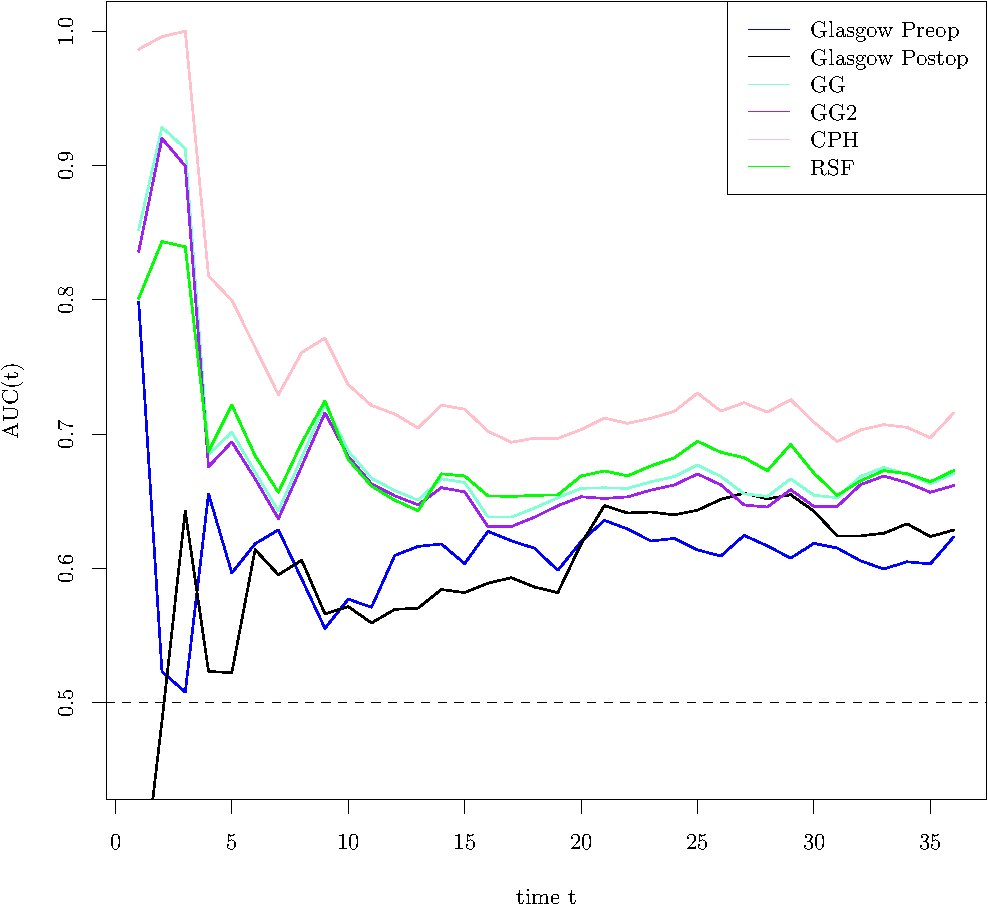
\includegraphics[width=\maxwidth]{figure/05-timeROC-1} 

}



\end{knitrout}

\begin{knitrout}
\definecolor{shadecolor}{rgb}{0.969, 0.969, 0.969}\color{fgcolor}\begin{kframe}
\begin{alltt}
\hlcom{# invisible(risksetROC(data.glasgow$Time/365.25*12, status = data.glasgow$DSD, marker = mskcc_pre.linpred.glasgow, predict.time = 12))}
\hlcom{# invisible(risksetROC(data.glasgow$Time/365.25*12, status = data.glasgow$DSD, marker = mskcc_post.linpred.glasgow, predict.time = 12))}
\hlcom{# invisible(risksetROC(data.glasgow$Time/365.25*12, status = data.glasgow$DSD, marker = gg.linpred.glasgow, predict.time = 12))}
\hlcom{# invisible(risksetROC(data.glasgow$Time/365.25*12, status = data.glasgow$DSD, marker = cph.linpred.glasgow, predict.time = 12))}
\hlcom{# invisible(risksetROC(data.glasgow$Time/365.25*12, status = data.glasgow$DSD, marker = rsf.linpred.glasgow, predict.time = 12))}
\hlkwd{invisible}\hlstd{(}\hlkwd{risksetAUC}\hlstd{(data.glasgow}\hlopt{$}\hlstd{Time}\hlopt{/}\hlnum{365.25}\hlopt{*}\hlnum{12}\hlstd{,} \hlkwc{status} \hlstd{= data.glasgow}\hlopt{$}\hlstd{DSD,} \hlkwc{marker} \hlstd{= mskcc_pre.linpred.glasgow,} \hlkwc{tmax} \hlstd{=} \hlnum{36}\hlstd{,} \hlkwc{col} \hlstd{= pal[}\hlstr{"mskcc.pre"}\hlstd{],} \hlkwc{lwd} \hlstd{=} \hlnum{2}\hlstd{))}
\hlkwd{par}\hlstd{(}\hlkwc{new} \hlstd{=} \hlnum{TRUE}\hlstd{)}
\hlkwd{invisible}\hlstd{(}\hlkwd{risksetAUC}\hlstd{(data.glasgow}\hlopt{$}\hlstd{Time}\hlopt{/}\hlnum{365.25}\hlopt{*}\hlnum{12}\hlstd{,} \hlkwc{status} \hlstd{= data.glasgow}\hlopt{$}\hlstd{DSD,} \hlkwc{marker} \hlstd{= mskcc_post.linpred.glasgow,} \hlkwc{tmax} \hlstd{=} \hlnum{36}\hlstd{,} \hlkwc{col} \hlstd{= pal[}\hlstr{"mskcc.post"}\hlstd{],} \hlkwc{lwd} \hlstd{=} \hlnum{2}\hlstd{))}
\hlkwd{par}\hlstd{(}\hlkwc{new} \hlstd{=} \hlnum{TRUE}\hlstd{)}
\hlkwd{invisible}\hlstd{(}\hlkwd{risksetAUC}\hlstd{(data.glasgow}\hlopt{$}\hlstd{Time}\hlopt{/}\hlnum{365.25}\hlopt{*}\hlnum{12}\hlstd{,} \hlkwc{status} \hlstd{= data.glasgow}\hlopt{$}\hlstd{DSD,} \hlkwc{marker} \hlstd{= gg.linpred.glasgow,} \hlkwc{tmax} \hlstd{=} \hlnum{36}\hlstd{,} \hlkwc{col} \hlstd{= pal[}\hlstr{"gg"}\hlstd{],} \hlkwc{lwd} \hlstd{=} \hlnum{2}\hlstd{))}
\hlkwd{par}\hlstd{(}\hlkwc{new} \hlstd{=} \hlnum{TRUE}\hlstd{)}
\hlcom{# invisible(risksetAUC(data.glasgow$Time/365.25*12, status = data.glasgow$DSD, marker = cph.linpred.glasgow, tmax = 36, col = pal["cph"], lwd = 2))}
\hlcom{# par(new = TRUE)}
\hlcom{# invisible(risksetAUC(data.glasgow$Time/365.25*12, status = data.glasgow$DSD, marker = rsf.linpred.glasgow, tmax = 36, col = pal["rsf"], lwd = 2))}
\hlcom{# legend("top", legend = c("Glasgow Preop", "Glasgow Postop", "GG", "CPH", "RSF"), col = c(pal["mskcc.pre"], pal["mskcc.post"], pal["gg"], pal["cph"], pal["rsf"]), lty = "solid", lwd = 2)}
\hlkwd{legend}\hlstd{(}\hlstr{"top"}\hlstd{,} \hlkwc{legend} \hlstd{=} \hlkwd{c}\hlstd{(}\hlstr{"Glasgow Preop"}\hlstd{,} \hlstr{"Glasgow Postop"}\hlstd{,} \hlstr{"GG"}\hlstd{),} \hlkwc{col} \hlstd{=} \hlkwd{c}\hlstd{(pal[}\hlstr{"mskcc.pre"}\hlstd{], pal[}\hlstr{"mskcc.post"}\hlstd{], pal[}\hlstr{"gg"}\hlstd{]),} \hlkwc{lty} \hlstd{=} \hlstr{"solid"}\hlstd{,} \hlkwc{lwd} \hlstd{=} \hlnum{2}\hlstd{)}
\hlkwd{abline}\hlstd{(}\hlkwc{v} \hlstd{=} \hlkwd{c}\hlstd{(}\hlnum{7}\hlstd{,} \hlnum{31}\hlstd{))}
\end{alltt}
\end{kframe}

{\centering 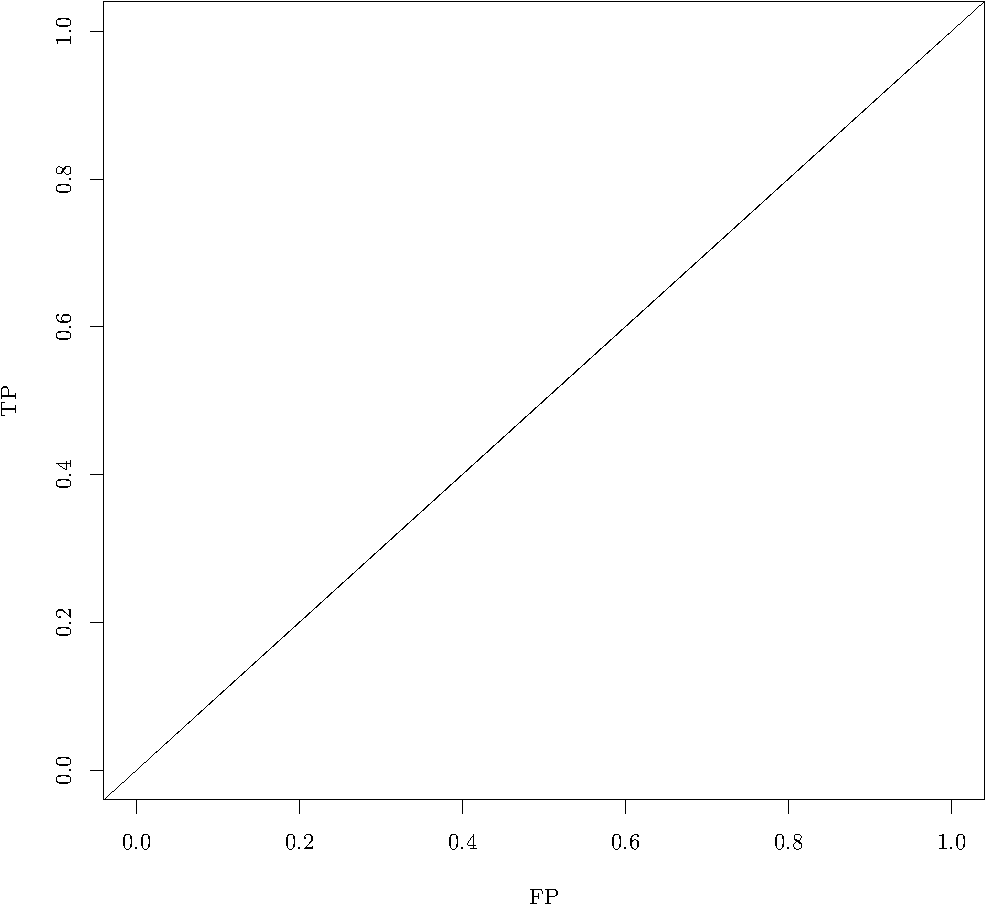
\includegraphics[width=\maxwidth]{figure/05-risksetROC-1} 

}



\end{knitrout}

\end{document}
